\vspace{15cm}
\chapter{Jaringan Saraf Fuzzy} \label{bab jsf}

\noindent Jaringan saraf fuzzy (\gls{jsf}) dapat dipandang sebagai jaringan saraf tiruan (JST) yang lapisan tersembunyi dan lapisan keluarannya merupakan hasil dari langkah-langkah dalam sistem kontrol logika fuzzy. Keluaran dari sistem kontrol logika fuzzy berupa tindakan kontrol. Sistem kontrol logika fuzzy akan dijelaskan pada Subbab \ref{flc}. Sama seperti JST, JSF juga menghasilkan suatu model. Tetapi, model yang dihasilkan berupa sistem kontrol logika fuzzy tertentu sedemikian sehingga dapat meminimalkan galat antara tindakan kontrol dan keluaran yang diinginkan. Untuk meminimalkan galat ini, dibutuhkan suatu konstruksi JSF yang tepat. Konstruksi ini akan melalui tahapan-tahapan tertentu yang akan dijelaskan pada Subbab \ref{konst fnn}. Sebelum membahas sistem kontrol logika fuzzy dan konstruksi JSF, bab ini akan membahas konsep dasar fuzzy terlebih dahulu. Konsep dasar ini meliputi himpunan fuzzy beserta operasinya yang akan dijelaskan pada Subbab \ref{himpunan fuzzy} dan \ref{op h fuzzy}. Selanjutnya, akan dijelaskan logika fuzzy pada Subbab \ref{logika fuzzy} yang meliputi negasi, konjungsi, disjungsi, dan implikasi. Pembahasan pada tiga subbab pertama akan menggunakan pendekatan konsep dasar himpunan klasik dan logika klasik. Subbab \ref{fuzzy rules infer} akan membahas aturan fuzzy dan inferensi fuzzy yang keduanya memiliki peranan yang sangat penting dalam sistem kontrol logika fuzzy.

%%%%-----HIMPUNAN FUZZY------
\section{Himpunan Fuzzy} \label{himpunan fuzzy}
\noindent Perbedaan antara himpunan klasik dan himpunan fuzzy terletak pada tegas atau tidaknya sifat keanggotaan. Pada himpunan klasik, keanggotaannya bersifat tegas. Sedangkan keanggotaan dari himpunan fuzzy bersifat tidak tegas atau kabur.

\noindent Misalkan himpunan klasik $C$ didefinisikan oleh $C=\{3k : k\in\gls{z} \}$ atau himpunan yang terdiri dari bilangan bulat yang merupakan kelipatan dari $3$. Maka $6$ adalah anggota himpunan klasik $C$ dan $7$ bukan anggota himpunan klasik $C$. Nilai kebenaran dari keanggotaan suatu himpunan klasik hanya dapat direpresentasikan oleh nilai benar atau salah. Pernyataan ``$6$ adalah anggota himpunan klasik $C$'' bernilai benar. Pernyataan ``$7$ adalah anggota himpunan klasik $C$'' bernilai salah. Berdasarkan nilai kebenaran ini, dapat dibangun fungsi indikator dari himpunan klasik $C$ yang mendefinisikan apakah suatu anggota $\mathbb{Z}$ adalah anggota himpunan $C$ atau bukan. Misalkan $f_C$ adalah fungsi indikator dari himpunan klasik $C$. Maka $f_C$ didefinisikan oleh
\begin{align*}
    f_C(x)=
    \begin{dcases}
    1, & \text{jika } x \in C\\
    0, & \text{jika } x \notin C
    \end{dcases}
\end{align*}
untuk setiap $x \in \mathbb{Z}$.

\noindent Keanggotaan himpunan fuzzy bergantung pada suatu fungsi keanggotaannya. Misalkan himpunan fuzzy $A$ terdiri dari bilangan real yang dekat dengan $3$. Maka $3$, $5$, dan $10$ adalah anggota himpunan fuzzy $A$, tetapi dengan nilai fungsi keanggotaan yang berbeda-beda. Bilangin real yang lebih dekat dengan $3$ akan memiliki nilai fungsi keanggotaan yang lebih besar. Bilangan real $100$ juga anggota himpunan fuzzy $A$, tetapi dengan nilai fungsi keanggotaan yang cukup kecil. Jika nilai pernyataan yang benar dan salah berturut-turut diwakili oleh $1$ dan $0$, maka nilai kebenaran dari keanggotaan suatu himpunan fuzzy dapat direpresentasikan oleh bilangan real dari $0$ sampai dengan $1$. Pernyataan ``$3$ adalah anggota himpunan fuzzy $A$'' memiliki nilai kebenaran yang lebih besar dari pernyataan ``$\num{2,5}$ adalah anggota himpunan fuzzy $A$''.

\noindent Himpunan fuzzy telah diperkenalkan oleh \citeasnoun{zadeh}. Pendefinisian himpunan fuzzy ditulis secara formal oleh \citeasnoun{fuller}.

\begin{definition}
\label{fuzzyset}
Misalkan $X$ adalah himpunan takkosong. Sebuah himpunan fuzzy $A$ di $X$ dikarakterisasi oleh fungsi keanggotaannya, yaitu
\[ \gls{mu}: X \rightarrow [0,1] \]
dan $\mu_A(x)$ diinterpretasikan sebagai derajat keanggotaan dari elemen $x$ di himpunan fuzzy $A$ untuk setiap $x \in X$.
\end{definition}

\noindent Berdasarkan Definisi \ref{fuzzyset}, himpunan fuzzy $A$ di $X$ dapat ditulis sebagai
\[A = \{ \left(x,\mu_A(x)\right) : x \in X \}.\]
Contoh \ref{contoh: himp fuzzy} bertujuan supaya konsep himpunan fuzzy dan fungsi keanggotaanya di bilangan real dapat lebih mudah dipahami.

\begin{contoh} \label{contoh: himp fuzzy}
Misalkan himpunan fuzzy $A$ di $\gls{real}$ terdiri dari bilangan real $x$ yang dekat dengan $3$ dan didefinisikan oleh $A= \left\{ \left(x,\mu_A(x)\right) : x \in \mathbb{R} \right\}$ dengan
\[\mu_A(x) =
\begin{dcases}
1+\displaystyle\frac{x-3}{10}, & -7 \leq x \leq 3\\
1-\displaystyle\frac{x-3}{10}, & 3 < x \leq 13\\
0, & x \text{ lainnya.}
\end{dcases}
\]
Grafik dari fungsi keanggotaan $\mu_A$ ini dapat dilihat pada \ref{figFuzzy3}. Berdasarkan grafik tersebut, jelas bahwa $3$ memiliki derajat keanggotaan yang paling besar, yaitu $\mu_A(3)=1$. 
\end{contoh}

\begin{figure}[htbp!]
    \centering
    \begin{tikzpicture}
    \begin{axis}[axis lines = middle, xlabel = $x$,
            every axis x label/.style={
                at={(ticklabel* cs:1.05)},
                anchor=west,
            },
            xmin=-8, xmax=14,
            ymin=0, ymax=1.2,
            minor tick num=2,
            xtick={-7,3,13}, ytick={0,1},]
        \addplot [domain=-7:3,samples=100,color=black,]{1+(x-3)/10};
        \addplot [domain=3:13,samples=100,color=black,]{1-(x-3)/10};
    \end{axis}
    \end{tikzpicture}
    \caption{Fungsi keanggotaan untuk ``$x$ dekat dengan $3$''}
    \label{figFuzzy3}
\end{figure}

%%%%-----OPERASI PADA HIMPUNAN FUZZY------
\section{Operasi pada Himpunan Fuzzy} \label{op h fuzzy}
\noindent Pada himpunan klasik, terdapat operasi irisan, gabungan, dan komplemen. Misalkan $C$ dan $D$ adalah himpunan klasik di $X$. Irisan dari $C$ dan $D$ ($C \gls{irisan} D$) menyatakan himpunan yang setiap anggotanya adalah anggota dari himpunan $C$ sekaligus anggota dari himpunan $D$. Setiap anggota dari gabungan himpunan $C$ dan $D$ ($C \gls{gabungan} D$) adalah anggota dari himpunan $C$ atau anggota dari himpunan $D$. Komplemen dari himpunan $D$ ($D\gls{kom}$) terdiri dari anggota himpunan semesta $X$, tetapi bukan anggota himpunan $D$. Jika dibangun fungsi keanggotaan dari $C \cap D$, $C \cup D$, dan $D^C$, maka untuk setiap $x \in X$ berlaku
\begin{align*}
    f_{C \cap D}(x) &= 
    \begin{dcases}
        1, & \text{jika } f_C(x) = 1 \text{ dan } f_D(x) = 1\\
        0, & x \text{ lainnya}
    \end{dcases}
    \\
    f_{C \cup D}(x) &= 
    \begin{dcases}
        1, & \text{jika } f_C(x) = 1 \text{ atau } f_D(x) = 1\\
        0, & x \text{ lainnya}
    \end{dcases}
    \\
    f_{D^C}(x) &= 
    \begin{dcases}
        1, & \text{jika } f_D(x) = 0\\
        0, & x \text{ lainnya}
    \end{dcases}
\end{align*}
Berdasarkan ketentuan di atas, maka fungsi keanggotaan $f_{C \cap D}$, $f_{C \cup D}$, dan $f_{D^C}$ juga dapat ditulis dengan cara sebagai berikut:
\begin{align}
    \label{fkk1}
    f_{C \cap D}(x) &= \min \{f_C(x),f_D(x) \}= f_C(x)f_D(x)\\
    \label{fkk2}
    f_{C \cup D}(x) &= \maks \{f_C(x),f_D(x) \}= f_C(x)+f_D(x)-f_C(x)f_D(x)\\
    \label{fkk3}
    f_{D^C}(x) &= 1-f_D(x)
\end{align}

\noindent Himpunan fuzzy mempunyai operasi komplemen, irisan dan gabungan juga. Karena keanggotaan himpunan fuzzy bersifat tidak tegas dan bergantung kepada fungsi keanggotaannya, maka setiap himpunan fuzzy yang dihasilkan dari pengoperasian himpunan-himpunan fuzzy mempunyai fungsi keanggotaannya sendiri. Definisi fungsi keanggotaan dari komplemen suatu himpunan fuzzy sesuai dengan Persamaan (\ref{fkk3}). Fungsi keanggotaan dari irisan dan gabungan himpunan-himpunan fuzzy  berturut-turut didefinisikan oleh \emph{\gls{tnorm}} dan \emph{\gls{tconorm}}. Dalam teori himpunan fuzzy, \textit{t-norm} dan \textit{t-conorm} berturut-turut digunakan untuk memodelkan nilai kebenaran dari konjungsi dan disjungsi pada suatu pernyataan \cite{fuller}.
\begin{definition}[\emph{t-norm}]\label{tnorm}
Pemetaan $\gls{T}: [0,1] \times [0,1] \to [0,1]$ disebut \textit{t-norm} jika dan hanya jika memenuhi sifat-sifat berikut ini:
\begin{itemize}
    \item $T(x,y) = T(y,x) \quad \forall x,y \in [0,1]$ (simetri)
    \item $T\left(x,T(y,z)\right) = T\left(T(x,y),z\right) \quad \forall x,y,z \in [0,1]$ (asosiatif)
    \item $T(x,y) \leq T(x',y') \quad \forall x,y,x',y' \in [0,1]$ dengan $x \leq x'$ dan $y \leq y'$ (monoton)
    \item $T(x,1) = x \quad \forall x \in[0,1]$ (satu sebagai elemen identitas)
\end{itemize}
\end{definition}

\noindent

\begin{definition}[\emph{t-conorm}]\label{tconorm}
Pemetaan $\gls{S}: [0,1] \times [0,1] \to [0,1]$ disebut \textit{t-conorm} jika dan hanya jika memenuhi sifat-sifat berikut ini:
\begin{itemize}
    \item $S(x,y) = S(y,x) \quad \forall x,y \in [0,1]$ (simetri)
    \item $S\left(x,S(y,z)\right) = S\left(S(x,y),z\right) \quad \forall x,y,z \in [0,1]$ (asosiatif)
    \item $S(x,y) \leq S(x',y') \quad \forall x,y,x',y' \in [0,1]$ dengan $x \leq x'$ dan $y \leq y'$ (monoton)
    \item $S(x,0) = x \quad \forall x \in[0,1]$ (nol sebagai elemen identitas)
\end{itemize}
\end{definition}

\noindent Misalkan $T$ adalah \emph{t-norm}. Misalkan \emph{t-conorm} $S$ memenuhi persamaan $S(a,b) = 1 - T(1-a,1-b)$ untuk setiap $a,b \in [0,1]$. Maka dapat dikatakan bahwa $S$ diturunkan dari $T$ \cite{fuller}.

\noindent Berdasarkan Definisi \ref{tnorm} dan \ref{tconorm}, maka muncul beberapa pasangan operator \emph{t-norm} dan \emph{t-conorm} dasar. Pada \ref{basic_t_norm} ditampilkan beberapa pasangan \emph{t-norm} dan \emph{t-conorm} dasar yang cukup sering digunakan.

\begin{table}[h!]
\centering
\caption[Tabel \emph{t-norm} dan \emph{t-conorm} dasar]{Tabel \emph{t-norm} dan \emph{t-conorm} dasar \protect\cite{fuller}} 
\label{basic_t_norm}
\begin{tabular}{lll} 
\toprule
\multicolumn{1}{c}{ } & \multicolumn{1}{c}{\emph{T-norm}}  & \multicolumn{1}{c}{\emph{T-conorm}}\\ [0.5ex]
\multicolumn{1}{c}{ } & \multicolumn{1}{c}{$\left(T(a,b)\right)$}  & \multicolumn{1}{c}{$\left(S(a,b)\right)$}\\
 \midrule
 Minimum Maksimum & $\min \{a,b\}$ &  $\maks \{a,b\}$ \\
 \L ukasiewicz & $\maks \{a+b-1,0\}$ &  $\min \{a+b,1\}$ \\
 Probabilistik & $ab$ &  $a+b-ab$ \\
 \bottomrule
\end{tabular}
\end{table}

\noindent Perhatikan bahwa \emph{t-norm} minimum dan probabilistik sesuai dengan Persamaan (\ref{fkk1}), serta \emph{t-conorm} maksimum dan probabilistik sesuai dengan Persamaan (\ref{fkk2}). Karena operasi irisan berkaitan dengan konjungsi dan \emph{t-norm} analog dengan Persamaan (\ref{fkk1}) yang merupakan fungsi keanggotaan dari irisan himpunan klasik, maka \emph{t-norm} dapat dijadikan sebagai derajat kebenaran suatu konjungsi dari pernyataan-pernyataan logika yang bersifat fuzzy, yaitu pernyataan yang nilai kebenarannya berada pada selang $[0,1]$. Dengan menggunakan argumen yang serupa dan bersesuaian, \emph{t-conorm} juga dapat dijadikan sebagai derajat kebenaran suatu disjungsi dari pernyataan-pernyataan logika yang bersifat fuzzy. Dengan demikian, \emph{t-norm} dan \emph{t-conorm} sangat tepat digunakan untuk mendefinisikan fungsi keanggotaan dari irisan dan gabungan himpunan fuzzy.
\begin{definition}[Irisan, gabungan dan komplemen pada himpunan fuzzy]\label{opfuzzy}
Misalkan $A$ dan $B$ adalah himpunan fuzzy di $X$ dengan fungsi keanggotaan $\mu_A$ dan $\mu_B$ berturut-turut. Maka fungsi keanggotaan dari $A \cap B$, $A \cup B$, dan $A^C$ berturut-turut didefinisikan oleh
\begin{align*}
    \mu_{A \cap B}(x) &= T\left(\mu_A(x),\mu_B(x)\right) \quad \forall x \in X\\
    \mu_{A \cup B}(x) &= S\left(\mu_A(x),\mu_B(x)\right) \quad \forall x \in X\\
    \mu_{A^C}(x) &= 1-\mu_A(x) \quad \forall x \in X
\end{align*}
dengan $T$ adalah \textit{t-norm} dan $S$ adalah \textit{t-conorm} yang diturunkan dari $T$.
\end{definition}

\noindent Contoh \ref{contoh: operasi himp fuzzy} dapat memberikan gambaran mengenai operasi irisan, gabungan, dan komplemen pada himmpunan fuzzy.

\begin{contoh} \label{contoh: operasi himp fuzzy}
Misalkan diberikan himpunan fuzzy $M$ dan $B$ di $\gls{r+}$. Himpunan fuzzy $M$ dan $B$ ini menyatakan volume dari suatu gas ideal. Himpunan fuzzy $M$ menyatakan volume ``sedang'', sedangkan himpunan fuzzy $B$ menyatakan volume ``besar''. Misalkan
$\mu_M(v)=\exp\left[-\left(\displaystyle \frac{v-20}{5} \right)^2 \right]$ dan
$\mu_B(v)=\displaystyle\frac{1}{1+\exp\left(23-v\right)}$ untuk setiap $v \in \mathbb{R}^+$
adalah fungsi keanggotaan dari himpunan fuzzy $M$ dan $B$ berturut-turut.
\begin{itemize}
    \item Jika operasi t-norm yang digunakan adalah t-norm probabilistik, maka diperoleh $M \cap B = \left\{\left(v,\mu_{M \cap B}(v)\right) : v \in \mathbb{R}^+ \right\}$ dengan 
    \begin{align*}
        \mu_{M \cap B}(v) &=
        T\left(\mu_M(v),\mu_B(v)\right) = \mu_M(v)\mu_B(v)\\
        &= \displaystyle\frac{\exp\left[-\left(\displaystyle \frac{v-20}{5} \right)^2 \right]} {1+\exp\left(23-v\right)}.
    \end{align*}
    Akibatnya, operasi t-conorm yang mendefinisikan fungsi keanggotaan dari gabungan himpunan fuzzy $M$ dan $B$ haruslah menggunakan t-conorm probabilistik juga. Maka diperoleh
    $M \cup B = \left\{\left(v,\mu_{M \cup B}(v)\right) : v \in \mathbb{R}^+ \right\}$ dengan
    \begin{align*}
        \mu_{M \cup B}(v) &=
        S\left(\mu_M(v),\mu_B(v)\right) = \mu_M(v) + \mu_B(v) - \mu_M(v)\mu_B(v)\\
        &= \displaystyle\frac{1+\exp\left[23-v-\left(\displaystyle \frac{v-20}{5} \right)^2 \right]} {1+\exp\left(23-v\right)}.
    \end{align*}
    
    \item Jika operasi t-norm yang digunakan adalah operasi minimum, maka diperoleh $M \cap B = \left\{\left(v,\mu_{M \cap B}(v)\right) : v \in \mathbb{R}^+ \right\}$ dengan 
    \begin{align*}
        \mu_{M \cap B}(v) &=
        T\left(\mu_M(v),\mu_B(v)\right) = \min\left\{\mu_M(v),\mu_B(v)\right\}\\
        &=
        \begin{dcases}
        \mu_B(v) = \displaystyle\frac{1}{1+\exp\left(23-v\right)}, & 0 < v \leq \num{23,4758}\\
        \mu_M(v) = \exp\left[-\left(\displaystyle \frac{v-20}{5} \right)^2 \right], & v > \num{23,4758}.
        \end{dcases}
    \end{align*}
    Akibatnya, operasi t-conorm yang mendefinisikan fungsi keanggotaan dari gabungan himpunan fuzzy $M$ dan $B$ haruslah menggunakan operasi maksimum. Maka diperoleh
    $M \cup B = \left\{\left(v,\mu_{M \cup B}(v)\right) : v \in \mathbb{R}^+ \right\}$ dengan
    \begin{align*}
        \mu_{M \cup B}(v) &=
        S\left(\mu_M(v),\mu_B(v)\right) = \maks\left\{\mu_M(v),\mu_B(v)\right\}\\
        &=
        \begin{dcases}
        \mu_M(v) = \exp\left[-\left(\displaystyle \frac{v-20}{5} \right)^2 \right], & 0 < v \leq \num{23,4758}\\
        \mu_B(v) = \displaystyle\frac{1}{1+\exp\left(23-v\right)}, & v > \num{23,4758}.
        \end{dcases}
    \end{align*}
    \item Misalkan himpunan fuzzy $B^C$ di $\mathbb{R}^+$ menyatakan volume yang ``tidak besar'' dari suatu gas ideal. Maka fungsi keanggotaan $\mu_{B^C}$ adalah
    \begin{align*}
        \mu_{B^C}(v) &= 1 - \mu_B(v) = 1 - \displaystyle\frac{1}{1+\exp\left(23-v\right)}\\
        &= \displaystyle\frac{1}{1+\exp\left(v-23\right)}.
    \end{align*}
\end{itemize}
\end{contoh}


%%%%-----LOGIKA FUZZY------
\section{Logika Fuzzy} \label{logika fuzzy}
\noindent Nilai kebenaran suatu pernyataan pada logika klasik dapat dinyatakan dengan $1$ untuk nilai ``benar'' dan $0$ untuk nilai ``salah''. Misalkan $p$ dan $q$ adalah pernyataan logika klasik dengan
\begin{align}
    \label{p}
    p &:\text{``}x \text{ adalah anggota himpunan }C\text{''} \Leftrightarrow \text{``}x \in C \text{''}\\
    \label{q}
    q &:\text{``}y \text{ adalah anggota himpunan }D\text{''} \Leftrightarrow \text{``}y \in D \text{''}
\end{align}
Himpunan $C$ dan himpunan $D$ di sini adalah himpunan klasik. Misalkan $\tau(\cdot)$ menyatakan derajat kebenaran suatu pernyataan logika klasik. Maka $\tau(p)=1$ dan $\tau(q)=1$ ketika $x \in C$ dan $y \in D$. Jika $x \notin C$ atau pernyataan $p$ bernilai salah maka $\tau(p)=0$, dan jika $y \notin D$ maka $\tau(q)=0$.

\noindent Berdasarkan pernyataan logika klasik $p$ yang didefinisikan pada (\ref{p}), maka negasi dari pernyataan $p$ adalah
\[\gls{neg} p : \text{ ``}x \text{ bukan anggota himpunan }C \text{''} \Leftrightarrow \text{``}x \notin C \text{''} \]
Ketika pernyataan $\neg p$ bernilai benar atau ``$x \notin C$'', maka $\tau(\neg p)=1$. Jika $x \notin C$, maka pernyataan $p$ bernilai salah, sehingga $\tau(p)=0$. Ketika pernyataan $\neg p$ bernilai salah atau ``$x \in C$'', maka $\tau(\neg p)=0$. Jika $x \in C$, maka pernyataan $p$ bernilai benar, sehingga $\tau(p)=1$. Dengan demikian, derajat kebenaran dari pernyataan $\neg p$ dapat dinyatakan dengan
\begin{align} \label{negasi}
    \tau(\neg p) = 1 - \tau(p)
\end{align}

\noindent Nilai kebenaran suatu pernyataan pada logika fuzzy dapat dinyatakan dengan bilangan real pada selang $[0,1]$. Misalkan $A$ adalah himpunan fuzzy di $X$ dan $B$ adalah himpunan fuzzy di $Y$. Misalkan  fungsi keanggotaan dari himpunan fuzzy $A$ dan $B$ berturut-turut adalah $\mu_A$ dan $\mu_B$. Misalkan pernyataan logika fuzzy $r$ dan $s$ 
didefinisikan sebagai 
\begin{align}
    \begin{split} \label{r}
    r &:\text{``}x \text{ adalah anggota dari himpunan fuzzy }A\text{''}\\
    &\Leftrightarrow x \text{ anggota }A
    \end{split}
    \\
    \begin{split} \label{s}
    s &:\text{``}y \text{ adalah anggota dari himpunan fuzzy }B\text{''}\\
    &\Leftrightarrow y \text{ anggota }B
    \end{split}
\end{align}
Maka dapat diinterpretasikan bahwa $r$ dan $s$ adalah pernyataan logika fuzzy dengan derajat kebenaran $\mu_A(x)$ dan $\mu_B(y)$ berturut-turut. Dengan kata lain, $\tau(r)=\mu_A(x)$ dan $\tau(s)=\mu_B(y)$. Pada pernyataan logika fuzzy, terdapat istilah-istilah penting, di antaranya:
\begin{itemize}
    \item Variabel linguistik, yaitu variabel yang nilainya berupa himpunan fuzzy atau variabel yang nilainya didefinisikan dalam istilah linguistik. Pada dua pernyataan logika fuzzy di atas, $x$ dan $y$ merupakan variabel linguistik.
    \item Nilai linguistik, yaitu himpunan fuzzy atau istilah linguistik yang mendeskripsikan variabel linguistik. Nilai linguistik dideskripsikan oleh fungsi keanggotaan himpunan fuzzy. Pada pernyataan $r$ dan $s$, $A$ dan $B$ adalah nilai linguistik dari variabel $x$ dan $y$ berturut-turut.
    \item Himpunan semesta, yaitu domain dari nilai linguistik. Pada pernyataan $r$, himpunan $X$ adalah himpunan semesta.
\end{itemize}

\noindent Misalkan $\neg r$ adalah negasi dari pernyataan logika fuzzy $r$. Maka $\neg r$ dapat diinterpretasikan sebagai ``$x$ adalah anggota dari himpunan fuzzy $A^C$''. Berdasarkan derajat kebenaran dari negasi suatu pernyataan logika klasik yang dinyatakan pada (\ref{negasi}) dan definisi dari komplemen suatu himpunan fuzzy pada Definisi \ref{opfuzzy}, maka derajat kebenaran dari pernyataan $\neg r$ dapat dinyatakan dengan
\[ \tau(\neg r) = 1 - \tau(r) = 1 - \mu_A(x) = \mu_{A^C}(x) \]

\noindent Derajat kebenaran dari konjungsi, disjungsi, dan implikasi fuzzy dapat ditentukan dengan menggunakan konsep perluasan dari konjungsi, disjungsi, dan implikasi pada logika klasik. Konjungsi dan disjungsi fuzzy akan dibahas pada Subbab \ref{kondis}. Implikasi fuzzy akan dibahas pada Subbab \ref{imp}.

\subsection{Konjungsi dan Disjungsi Fuzzy} \label{kondis}
\noindent Konjungsi yang melibatkan minimal dua pernyataan logika klasik disebut dengan konjungsi pokok. Misalkan $p \gls{konj} q$ adalah konjungsi pokok dengan pernyataan $p$ dan $q$ berturut-turut didefinisikan pada (\ref{p}) dan (\ref{q}). Konjungsi pokok $p \land q$ bernilai benar jika dan hanya jika pernyataan $p$ dan $q$ keduanya bernilai benar. Dengan demikian, derajat kebenaran $p \land q$ ditentukan oleh
\[
\tau(p \land q) = 
\begin{dcases}
1, & \text{jika } \tau(p) = \tau(q) = 1\\
0, & \text{lainnya}
\end{dcases}
\]
Berdasarkan ketentuan di atas, derajat kebenaran $p \land q$ juga dapat dinyatakan oleh
\begin{align}
    \label{konjungsi_c}
    \tau(p \land q) = \min\{\tau(p),\tau(q)\} = \tau(p)\tau(q) = \maks \{ \tau(p)+\tau(q)-1,0\}
\end{align}

\noindent Disjungsi yang melibatkan minimal dua pernyataan logika klasik disebut dengan disjungsi pokok. Misalkan $p \gls{disj} q$ adalah disjungsi pokok dengan pernyataan $p$ dan $q$ berturut-turut didefinisikan pada (\ref{p}) dan (\ref{q}). Disjungsi pokok $p \lor q$ bernilai benar jika dan hanya jika salah satu dari pernyataan $p$ dan $q$ bernilai benar. Dengan demikian, derajat kebenaran $p \lor q$ ditentukan oleh
\[
\tau (p \lor q) =
\begin{dcases}
1, & \text{jika } \tau(p)=1 \text{ atau } \tau(q)=1\\
0, & \text{lainnya}
\end{dcases}
\]
Berdasarkan ketentuan di atas, derjat kebenaran $p \lor q$ juga dapat dinyatakan oleh
\begin{align}
    \label{disjungsi_c}
    \begin{split}
        \tau (p \lor q) &= \maks \{ \tau(p),\tau(q)\} = \tau(p) + \tau(q) - \tau(p)\tau(q)\\
        &= \min \{\tau(p) + \tau(q), 1\}
    \end{split}
\end{align}

\noindent Konjungsi yang melibatkan minimal dua pernyataan logika fuzzy disebut dengan konjungsi fuzzy. Disjungsi yang melibatkan minimal dua pernyataan logika fuzzy juga disebut dengan disjungsi fuzzy. Misalkan $r$ dan $s$ adalah dua pernyataan logika fuzzy yang didefinisikan pada (\ref{r}) dan (\ref{s}) berturut-turut. Misalkan $r \land s$ dan $r \lor s$ berturut-turut adalah konjungsi dan disjungsi fuzzy. Maka derajat kebenaran dari $r \land s$ dan $r \lor s$ dapat ditulis
\begin{align*}
    \tau(r \land s) &= \mu_{A \land B}(x,y)\\
    \tau(r \lor s) &= \mu_{A \lor B}(x,y)
\end{align*}
Bentuk $A \land B$ dan $A \lor B$ di sini dapat dipandang sebagai himpunan fuzzy di $X \times Y$. Himpunan fuzzy $A \land B$ dan $A \lor B$ berturut-turut memiliki fungsi keanggotaan $\mu_{A \land B}$ dan $\mu_{A \lor B}$ yang keduanya memetakan $X \times Y$ terhadap selang $[0,1]$. Berdasarkan Persamaan (\ref{konjungsi_c}) dan (\ref{disjungsi_c}), maka perluasan dari konjungsi dan disjungsi pokok ke konjungsi dan disjungsi fuzzy adalah
\begin{align*}
    \mu_{A \land B}(x,y) &= T\left(\mu_A(x),\mu_B(y)\right)\\
    \mu_{A \lor B}(x,y) &= S\left(\mu_A(x),\mu_B(y)\right)
\end{align*}
dengan $T$ adalah \emph{t-norm} dan $S$ adalah \emph{t-conorm} yang diturunkan dari $T$.

\subsection{Implikasi Fuzzy} \label{imp}
\noindent Implikasi yang melibatkan minimal dua pernyataan logika klasik disebut dengan implikasi pokok. Misalkan $p \gls{im} q$ adalah implikasi pokok dengan $p$ dan $q=$ berturut-turut didefinisikan pada (\ref{p}) dan (\ref{q}). Pernyataan $p$ disebut sebagai bagian pendahulu dari implikasi pokok  $p \rightarrow q$ dan pernyataan $q$ disebut sebagai bagian konsekuensi dari $p \rightarrow q$. Interpertasi dari implikasi pokok $p \rightarrow q$ adalah bahwa derajat kebenaran dari $p \rightarrow q$ mengkuantifikasi sejauh mana $q$ setidaknya memiliki derajat kebenaran yang sama dengan $p$ \cite{fuller}, yaitu
\begin{align}
\label{truth_implikasi_p}
\tau (p \rightarrow q) = 
\begin{dcases}
1, & \text{jika } \tau(p) \leq \tau(q)\\
0, & \text{lainnya}
\end{dcases}    
\end{align}
Berdasarkan ketentuan derajat kebenaran ini, diperoleh \ref{implikasi_pokok}.
\begin{table}[h!]
    \centering
    \caption{Tabel kebenaran untuk implikasi pokok}
    \label{implikasi_pokok}
    \begin{tabular}{c c c}
        $\tau(p)$ & $\tau(q)$ & $\tau(p) \rightarrow \tau(q)$ \\
        \hline
         1 & 1 & 1\\
         0 & 1 & 1\\
         0 & 0 & 1\\
         1 & 0 & 0
    \end{tabular}
\end{table}

\noindent Implikasi yang melibatkan minimal dua pernyataan logika fuzzy disebut dengan implikasi fuzzy. Ketentuan derajat kebenaran implikasi pokok pada Persamaan (\ref{truth_implikasi_p}) dapat diperluas menjadi ketentuan untuk derajat kebenaran dari implikasi fuzzy. Misalkan pernyataan $r$ dan $s$ yang didefinisikan pada (\ref{r}) dan (\ref{s}) adalah dua pernyataan logika fuzzy. Misalkan pula $r \rightarrow s$ adalah implikasi fuzzy dan dapat dinyatakan dengan 
\[r \rightarrow s : \text{Jika } x \text{ adalah }A \text{, maka } y \text{ adalah }B\]
Pada implikasi fuzzy ini, terdapat istilah-istilah yang berasosiasi dengan istilah dalam pernyataan logika fuzzy dan implikasi pokok:
\begin{itemize}
    \item $x$ disebut sebagai variabel linguistik bagian pendahulu dengan nilai linguistik $A$,
    \item $y$ disebut sebagai variabel linguistik bagian konsekuensi dengan nilai linguistik $B$.
\end{itemize}
Derajat kebenaran dari $r \rightarrow s$ dapat ditulis $\tau(r\rightarrow s) = \mu_{A \rightarrow B}(x,y)$. Bentuk $A \rightarrow B$ di sini dapat dipandang sebagai himpunan fuzzy di $X\times Y$. Himpunan fuzzy $A \rightarrow B$ memiliki fungsi keanggotaan $\mu_{A \rightarrow B}$ yang merupakan pemetaan dari $X\times Y$ terhadap selang $[0,1]$. Berdasarkan Persamaan (\ref{truth_implikasi_p}), salah satu perluasan dari implikasi pokok ke implikasi fuzzy yang memungkinkan adalah
\begin{align*}
    \mu_{A \rightarrow B}(x,y) = 
    \begin{dcases}
    1, & \text{jika } \mu_A(x) \leq \mu_B(y)\\
    0, & \text{lainnya}
    \end{dcases}
\end{align*}
Operator implikasi fuzzy ini disebut dengan operator \emph{Standard Strict}.

\noindent Namun, operator implikasi fuzzy ini tidak tepat untuk diaplikasikan di dunia nyata. Sebagai contoh, misalkan $\mu_A(x_1)=\num{0,7}$ dan $\mu_B(y_1)=\num{0,7}$ untuk suatu $x_1 \in X$ dan $y_1 \in Y$. Maka berdasarkan definisi dari operator \emph{Standard Strict}, mengakibatkan
\[\mu_{A \rightarrow B}(x_1,y_1) = 1\]
Misalkan $\mu_B(y_2)=\num{0,699}$ untuk suatu $y_2 \in Y$.  Dapat diinterpretasikan bahwa derjat keanggotaan $y_2$ di $B$ adalah derjat keanggotaan $y_1$ di $B$ yang tidak dibulatkan ke dalam satu angka di belakang tanda koma. Selanjutnya, diperoleh
\[\mu_{A \rightarrow B}(x_1,y_2) = 0\]
Contoh ini menunjukkan bahwa perubahan kecil pada derajat keanggotaan dari bagian konsekuensi dapat menyebabkan penyimpangan besar pada nilai kebenaran dari implikasi fuzzy. Dengan kata lain, operator ini sangat sensitif terhadap pembulatan.

\noindent Implikasi pokok $p \rightarrow q$ ekivalen dengan $\neg p \lor q$. Oleh karena itu, derajat kebenaran dari $p \rightarrow q$ dapat dinyatakan oleh
\[\tau(p \rightarrow q) = \tau(\neg p \lor q) = \maks \{\tau(\neg p),\tau(q)\} = \maks \{1-\tau(p),\tau(q)\}\]
Dengan menggunakan  konsep perluasan, fungsi keanggotaan $\mu_{A \rightarrow B}$ juga dapat dinyatakan oleh
\[ \mu_{A \rightarrow B}(x,y) = \maks \{ 1-\mu_A(x), \mu_B(y) \}, \forall x \in X, y \in Y \]
Operator ini disebut operator implikasi \emph{Kleene-Dienes}.

\noindent Perhatikan bahwa derajat kebenaran implikasi pokok $p \rightarrow q$ dapat dinyatakan juga oleh
\[ \tau(p \rightarrow q) = \sup \left\{z\in\{0,1\} : \min\{\tau(p),z\} \leq \tau(q) \right\}\]
Dengan menggunakan konsep perluasan, fungsi keanggotaan $\mu_{A \rightarrow B}$ juga dapat dinyatakan oleh
\begin{align*}
    \mu_{A \rightarrow B}(x,y) &= \sup \left\{z\in [0,1] : \min\{\mu_A(x),z\} \leq \mu_B(y) \right\}\\
    &=
    \begin{dcases}
    1, & \text{jika } \mu_A(x) \leq \mu_B(y)\\
    \mu_B(y), & \text{lainnya}
    \end{dcases}
\end{align*}
untuk setiap $x \in X$ dan $y \in Y$. Operator ini disebut operator implikasi \emph{G$\Ddot{o}$del}.

\noindent Dalam aplikasi praktis, untuk memodelkan hubungan sebab-akibat antara variabel-variabel yang bersifat fuzzy sering digunakan operator implikasi \emph{Mamdani}. Operator ini secara sederhana mengambil nilai minimum dari derajat kebenaran bagian pendahulu dan derajat kebenaran bagian konsekuensi pada suatu implikasi fuzzy. Dengan kata lain, operator implikasi \emph{Mamdani} dapat dinyatakan oleh
\[ \mu_{A \rightarrow B}(x,y) = \min \{\mu_A(x), \mu_B(y) \}, \forall x \in X, y \in Y \]
Misalkan $\mu_A(x_3)=0$ dan $\mu_B(y_3)=0$ untuk suatu $x_3 \in X$ dan $y_3 \in Y$. Dengan menggunakan operator implikasi \emph{Mamdani}, diperoleh $ \mu_{A \rightarrow B}(x_3,y_3) = 0$. Dengan demikian, operator ini bukanlah perluasan yang benar dari implikasi pokok. Namun, dalam sistem yang berbasis pengetahuan, kita biasanya tidak tertarik dengan aturan fuzzy (kumpulan dari implikasi fuzzy)  yang bagian-bagian pendahulunya bernilai salah.

\begin{table}[h!]
    \centering
    \caption{Operator implikasi fuzzy}
    \label{imfuzzy}
    \begin{tabular}{| l l |}
        \hline
        Nama & Definisi \\
        \hline
        Zadeh & $\mu_{A \rightarrow B}(x,y) = \maks \left\{ 1-\mu_A(x), \min \{\mu_A(x),\mu_B(y)\} \right\}$\\
        \L ukasiewicz & $\mu_{A \rightarrow B}(x,y) = \min \left\{ 1, 1-\mu_A(x)+\mu_B(y) \right\}$\\
        Kleene-Dienes & $\mu_{A \rightarrow B}(x,y) = \maks \left\{1-\mu_A(x),\mu_B(y) \right\}$\\
        Mamdani & $\mu_{A \rightarrow B}(x,y) = \min \left\{ \mu_A(x),\mu_B(y) \right\}$\\
        Larsen & $\mu_{A \rightarrow B}(x,y) = \mu_A(x)\mu_B(y)$\\
        \emph{Standard Strict} & $\mu_{A \rightarrow B}(x,y) =
        \begin{dcases}
        1, & \text{jika } \mu_A(x) \leq \mu_B(y)\\
        0, & \text{lainnya}
        \end{dcases}$\\
        G$\mathrm{\Ddot{o}}$del & $\mu_{A \rightarrow B}(x,y) =
        \begin{dcases}
        1, & \text{jika } \mu_A(x) \leq \mu_B(y)\\
        \mu_B(y), & \text{lainnya}
        \end{dcases}$\\
        Gaines & $\mu_{A \rightarrow B}(x,y) = 
        \begin{dcases}
        1, & \text{jika } \mu_A(x) \leq \mu_B(y)\\
        \displaystyle\frac{\mu_B(y)}{\mu_A(x)}, & \text{lainnya}
        \end{dcases}$\\
        \hline
    \end{tabular}
\end{table}

\noindent Terdapat tiga jenis operator implikasi fuzzy, yaitu:
\begin{itemize}
    \item Implikasi-$S$, didefinisikan oleh
    \[\mu_{A \rightarrow B}(x,y) = S\left(\mu_{A^C}(x),\mu_B(y) \right) = S\left(1-\mu_A(x),\mu_B(y) \right)\]
    dengan $S$ adalah \emph{t-conorm}. Contoh dari implikasi-$S$ ini adalah implikasi \emph{\L ukasiewicz} dan \emph{Kleene-Dienes}.
    \item Implikasi-$R$, didefinisikan oleh
    \[\mu_{A \rightarrow B}(x,y) = \sup \left\{ z \in [0,1] : T(\mu_A(x),z) \leq \mu_B(y) \right\}\]
    dengan $T$ adalah \emph{t-norm}. Contoh dari implikasi-$R$ adalah implikasi \emph{G$\Ddot{o}$del} dan \emph{Gaines}.
    \item Implikasi \emph{t-norm}. Misalkan $T$ adalah \emph{t-norm}. Maka implikasi ini didefinisikan oleh
    \[\mu_{A \rightarrow B}(x,y) = T\left(\mu_A(x),\mu_B(y) \right)\]
    Walaupun implikasi ini tidak memenuhi sifat-sifat dari implikasi pokok, implikasi ini sering digunakan sebagai model dalam berbagai aplikasi logika fuzzy. Contoh dari implikasi \emph{t-norm} adalah implikasi \emph{Mamdani} dan \emph{Larsen}.
\end{itemize}
Pendefinisian dari semua contoh operator yang disebutkan di atas dapat dilihat pada \ref{imfuzzy}.

%%%%-----ATURAN FUZZY DAN INFERENSI FUZZY------
\section{Aturan Fuzzy dan Inferensi Fuzzy} \label{fuzzy rules infer}
\noindent Aturan fuzzy terdiri dari kumpulan implikasi-implikasi fuzzy yang saling berkaitan. Bagian pendahulu dan bagian konsekuensi pada setiap implikasi dalam aturan fuzzy merupakan pernyataan logika fuzzy. Aturan fuzzy memiliki dua struktur umum yang berbeda, yaitu:
\begin{itemize}
    \item aturan fuzzy Zadeh yang digagas oleh \citeasnoun{zadeh73}, dan
    \item aturan fuzzy Takagi-Sugeno-Kang (\gls{tsk}) yang digagas oleh \citeasnoun{TakagiSugeno} dan \citeasnoun{SugenoKang}.
\end{itemize}
Perbedaan dari dua struktur ini terletak pada bagian konsekuensi. Pada aturan fuzzy Zadeh, setiap pernyataan yang berada di dalam bagian konsekuensi merupakan pernyataan logika fuzzy. Pada aturan fuzzy TSK, bagian konsekuensi dari setiap implikasinya berupa fungsi dari variabel-variabel linguistik pada bagian pendahulu.

\noindent Misalkan $A_{1,j},A_{2,j},\ldots,A_{m,j}$ adalah himpunan fuzzy di $X_j$ dengan $j=1,2,\ldots,n$ dan $x_1,x_2,...,x_n$ adalah variabel linguistik bagian pendahulu. Misalkan juga diberikan aturan fuzzy Zadeh dengan implikasi fuzzy sebanyak $m$. Variabel linguistik pada bagian konsekuensi hanya ada satu, yaitu $y$, dengan nilai linguistik $B_1,B_2,...,B_m$ pada himpunan semesta $Y$. Maka aturan fuzzy ini akan berbentuk
\generalFrZadeh%[x][A][y][B][n][3]
dengan \gls{fr} adalah aturan fuzzy ke-$i$.

\noindent Misalkan diberikan aturan fuzzy TSK yang terdiri dari sebanyak $m$ implikasi fuzzy. Misalkan pula fungsi pada bagian konsekuensi berupa fungsi yang linier terhadap variabel linguistik bagian pendahulu. Maka aturan fuzzy ini akan berbentuk
\generalFrTSK
dengan $\mathbf{b}_i = (b_{i,0}\textsc{, }b_{i,1}\textsc{, } b_{i,2}\textsc{, } \ldots\textsc{, } b_{i,n})$ untuk setiap $i=1, 2, \ldots, m$ dan $\mathbf{\Tilde{x}} = (1\textsc{, } x_1\textsc{, } x_2 \textsc{, } \ldots\textsc{, } x_n)$. Pada aturan fuzzy ini, bagian konsekuensi merupakan hasil dari operasi $\mathbf{b}_i\cdot\mathbf{\Tilde{x}}$. Maka variabel $y$ tidak terlihat seperti variabel linguistik karena tidak terlihat jelas sebagai anggota dari himpunan fuzzy. Tetapi, $\mathbf{b}_i\cdot\mathbf{\Tilde {x}}$ dapat dimodelkan sebagai himpunan fuzzy $B_i$, $i=1,2,\ldots,m$. Dengan demikian, menurut \citeasnoun{mendel} aturan fuzzy ini dapat dibuat menyerupai aturan fuzzy Zadeh dengan fungsi keanggotaan himpunan fuzzy $B_i$ adalah
\begin{align} \label{TSK kontrol}
    \mu_{B_i}(y) =
    \begin{dcases}
    1, & \text{jika } y=\mathbf{b}_i\cdot\mathbf{\Tilde{x}}\\
    0, & \text{lainnya}
    \end{dcases}
    \quad i=1,2,\ldots,m
\end{align}
Himpunan fuzzy $B_i$ ini disebut himpunan fuzzy diskrit. Hal ini dikarenakan
\[\left| \{y \in Y : \mu_{B_i}(y) > 0 \} \right| = 1 \in \gls{asli}.\]
Dengan kata lain, banyaknya anggota $Y$ yang derajat keanggotaannya positif di himpunan fuzzy $B_i$ adalah berhingga.

\noindent Inferensi klasik dikenal sebagai proses penarikan kesimpulan dari serangkaian fakta berdasarkan kumpulan aturan tertentu \cite{nedjah}. Salah satu jenis inferensi klasik adalah \emph{modus ponens}. Misalkan $p$ dan $q$ adalah pernyataan logika klasik yang didefinisikan pada (\ref{p}) dan (\ref{q}) berturut-turut. Misalkan diberikan
\begin{align*}
    \text{Aturan} &: \hspace{5px} p \rightarrow q &\\
    \text{Fakta} &: \hspace{5px} p
\end{align*}
Berdasarkan \emph{modus ponens}, diperoleh kesimpulan $q$.

\noindent Inferensi fuzzy adalah proses penarikan kesimpulan dari serangkaian fakta berdasarkan aturan fuzzy tertentu. Namun, serangkaian faktanya merupakan pernyataan-pernyataan logika fuzzy. Proses inferensi fuzzy juga menerapkan prinsip \emph{modus ponens} yang sama \cite{nedjah}. Mekanisme inferensi fuzzy akan dijelaskan pada Subbab \ref{flc}.

%%%%-----SISTEM KONTROL LOGIKA FUZZY------
\section{Sistem Kontrol Logika Fuzzy} \label{flc}
\noindent Sistem kontrol logika fuzzy (\gls{sklf}) adalah sistem kontrol yang berfungsi untuk mentransformasi serangkaian fakta menjadi suatu kesimpulan berupa tindakan kontrol berdasarkan aturan fuzzy tertentu melalui proses fuzzifikasi, inferensi fuzzy, dan defuzzifikasi. Bagian pendahulu pada setiap implikasi dalam aturan fuzzy dipandang sebagai suatu kondisi pada domain aplikasi sistem kontrol. Bagian konsekuensi pada setiap implikasi dalam aturan fuzzy dipandang sebagai tindakan kontrol untuk sistem yang dikendalikan. Oleh karena itu, pada SKLF, variabel linguistik bagian pendahulu disebut dengan variabel kondisi dan variabel linguistik bagian konsekuensi disebut variabel kontrol. Pada dasarnya, SKLF menyediakan cara yang mudah untuk mengekspresikan kebijakan kontrol dan domain pengetahuan \cite{fuller}.
\begin{figure}[htbp!]
    \centering
    \begin{tikzpicture}
    \small
    %Nodes
    \node (awal)   at (-4,-2)    {};
    \kotak[f,(-4,0)] {Fuzzifikasi};
    %\kotakbesar[60,180,kb,(3,-2)];
    \kotak[inffuzzy,(0,4)] {Inferensi Fuzzy};
    \kotak[fr,(0,0)] {Aturan Fuzzy};
    \kotak[df,(4,0)] {Defuzzifikasi};
    \node (akhir) at (4,-2) {};
     
    %Lines
    \singleT[awal,f,270,right]{Serangkaian fakta};
    \singleT[f,inffuzzy,0,above]{Himpunan-himpunan fuzzy};
    \singleT[inffuzzy,df,0,above]{Himpunan-himpunan fuzzy};
    \singleT[df,akhir,90,left]{Tindakan kontrol};
    \singleT[fr,inffuzzy,0,above]{};
    \singleT[fr,f,0,above]{};
    \end{tikzpicture}
    \caption{Sistem kontrol logika fuzzy}
    \label{fig:flc}
\end{figure}

\noindent Bentuk umum dari SKLF diberikan pada \ref{fig:flc}. SKLF terdiri dari empat bagian utama: fuzzifikasi, aturan fuzzy, inferensi fuzzy, dan defuzzifikasi. Pada tahap fuzzifikasi, serangkaian fakta yang bersifat nonfuzzy ditransformasi menjadi bilangan real pada selang $[0,1]$ menggunakan fungsi keanggotaan nilai linguistik dari variabel kondisi. Selanjutnya, dilakukan inferensi fuzzy terhadap hasil fuzzifikasi berdasarkan aturan fuzzy. Inferensi fuzzy ini akan menghasilkan himpunan fuzzy yang berpadanan dengan nilai linguistik dari variabel kontrol. Misalkan terdapat sebanyak $k$ variabel kontrol. Maka ada sebanyak $k$ nilai linguistik berupa himpunan fuzzy yang terlibat pada bagian konsekuensi dari setiap implikasinya. Akibatnya, himpunan fuzzy yang dihasilkan dari tahap ini ada sebanyak $k$. Inferensi fuzzy yang dilakukan pada tahap ini akan dijelaskan pada Bagian \ref{m inferensi f}. Pada akhirnya, dilakukan defuzzifikasi terhadap himpunan fuzzy yang dihasilkan dari tahap inferensi. Defuzzifikasi ini akan menghasilkan sebanyak $k$ tindakan kontrol. Metode-metode defuzzifikasi akan dijelaskan pada Bagian \ref{defuzz}.

\subsection{Metode Defuzzifikasi} \label{defuzz}
\noindent Defuzzifikasi adalah proses untuk memilih anggota yang mewakili himpunan fuzzy yang dihasilkan dari proses inferensi fuzzy \cite{fuller}. Defuzzifikasi akan menghasilkan keluaran yang bersifat nonfuzzy. Pada SKLF, hasil defuzzifikasi dipandang sebagai tindakan kontrol. Misalkan himpunan fuzzy $B$ di $Y$ dengan fungsi keanggotaan $\mu_B$ adalah hasil dari suatu proses inferensi fuzzy. Misalkan $\mathrm{defuzzifier}$ adalah operator defuzzifikasi. Maka diperoleh
\[ y_0 = \mathrm{defuzzifier}(\mu_B) \]
dengan $y_0$ adalah tindakan kontrol dari sistem kontrol logika fuzzy dan $y_0 \in Y$.

\noindent Operator defuzzifikasi yang sering digunakan adalah sebagai berikut:
\begin{itemize}
    \item \textbf{\emph{Center-of-Area/Gravity}.} Hasil defuzzifikasi dari himpunan fuzzy $B$ di $Y$ didefinisikan sebagai \emph{centroid} dari fungsi keanggotaan $\mu_B$, yaitu:
    \[y_0 = \displaystyle \frac{\int_Y y\mu_B(y)\dif y}{\int_Y \mu_B(y)\dif y}\]
    Jika $B$ adalah himpunan fuzzy diskrit, maka
    \[y_0 = \displaystyle \frac{\displaystyle\sum_{y \in Y} y\mu_B(y)}{\displaystyle\sum_{y \in Y} \mu_B(y)}\]
    \item \textbf{\emph{First-of-Maxima}.} Hasil defuzzifikasi dari himpunan fuzzy $B$ di $Y$ adalah elemen dengan nilai terkecil yang memaksimalkan $\mu_B$, yaitu:
    \[y_0 = \min\{y \in Y : y = \arg \underset{w \in Y}{\maks} \hspace{3px} \mu_B(w)\} \]
    \item \textbf{\emph{Middle-of-Maxima}.} Hasil defuzzifikasi dari himpunan fuzzy $B$ di $Y$ adalah rata-rata dari semua nilai nonfuzzy yang memaksimalkan $\mu_B$, yaitu:
    \[y_0 = \displaystyle \frac{\int_G y\dif y}{\int_G \dif y} \]
    dengan $G$ menyatakan himpunan bagian dari $Y$ yang elemen-elemennya memaksimalkan $\mu_B$, yaitu
    $G = \{y \in Y : \mu_B(y) = \underset{w}{\maks} \hspace{3px} \mu_B(w)\}$.
    Jika $G$ diskrit, maka
    \[y_0 = \displaystyle \frac{1}{|G|}\displaystyle\sum_{y\in G} y \]
    \item \textbf{\emph{Max-Criterion}.} Hasil defuzzifikasi dari himpunan fuzzy $B$ di $Y$ adalah sembarang elemen dari himpunan yang terdiri dari nilai nonfuzzy yang memaksimalkan $\mu_B$, yaitu:
    \[ y_0 \in \{y \in Y : y = \arg \underset{w\in Y}{\maks} \hspace{3px} \mu_B(w)\}\]
\end{itemize}

\subsection{Mekanisme Inferensi} \label{m inferensi f}
\noindent Berdasarkan struktur aturan fuzzy yang telah dijelaskan pada Subbab \ref{fuzzy rules infer}, maka ada dua mekanisme inferensi yang lazim digunakan dalam SKLF. Dua mekanisme inferensi ini adalah: mekanisme inferensi Mamdani dan mekanisme inferensi Takagi-Sugeno-Kang (TSK).

\subsubsection{Mekanisme Inferensi Mamdani}
\noindent Inferensi Mamdani merupakan inferensi fuzzy yang dilakukan terhadap aturan fuzzy Zadeh. Operator implikasi fuzzy yang digunakan pada inferensi ini adalah operator mamdani, yaitu operator minimum. Penghubung antar implikasi pada aturan fuzzy diinterpretasikan sebagai ``atau'', sehingga operator yang digunakan untuk menghubungkan semua implikasinya adalah operator maksimum.

\noindent Misalkan diberikan SKLF berikut ini
\flcmamdani
dengan $A_{1,j},A_{2,j}, \ldots, A_{m,j}$ adalah himpunan fuzzy di $X_j$ untuk setiap $j=1,2,\ldots,n$, dan $B_1, B_2, \ldots, B_m$ adalah himpunan fuzzy di $Y$. Variabel linguistik bagian pendahulu di sini adalah $x_1,x_2,\ldots,x_n$. Pada sistem kontrol ini hanya terdapat satu variabel linguistik bagian konsekuensi, yaitu $y$. Tugas utama dari SKLF ini adalah untuk memperoleh tindakan kontrol tertentu, yaitu nilai dari $y_0$.
Langkah-langkah untuk menyelesaikan sistem kontrol ini dengan menggunakan inferensi mamdani adalah sebagai berikut
\begin{enumerate}
\item Lakukan fuzzifikasi terhadap serangkaian fakta berdasarkan nilai linguistik dari variabel kondisi. Kemudian operasikan hasil fuzzifikasi tersebut dengan operasi konjungsi fuzzy (\emph{t-norm}). Misalkan hasil operasi ini dinyatakan dengan $\alpha_i$ untuk $i=1,2,\ldots m$. Maka diperoleh
\[\alpha_i = T\left( \mu_{A_{i,1}}(a_1),\mu_{A_{i,2}}(a_2),\ldots,\mu_{A_{i,n}}(a_n) \right)
\text{,} \quad i = 1,2,\ldots,m
\]
\item Operasikan bagian pendahulu dan bagian konsekuensi pada setiap implikasi menggunakan operator mamdani. Maka diperoleh sebanyak $m$ himpunan fuzzy baru di $Y$, yaitu himpunan fuzzy $B'_1, B'_2, \ldots, B'_m$ dengan fungsi keanggotaan
\[ \mu_{B'_i}(y) = \min \left\{ \alpha_i, \mu_{B_i}(y) \right\}
\text{,} \quad y \in Y \quad i = 1,2,\ldots,m
\]
\item Selanjutnya, dilakukan operasi \emph{t-conorm} untuk menggabungkan sebanyak $m$ himpunan fuzzy dari setiap implikasi. Maka diperoleh himpunan fuzzy baru di $Y$, yaitu himpunan fuzzy $B$ dengan fungsi keanggotaan
\[ \mu_B(y) = S\left(\mu_{B'_1}(y),\mu_{B'_2}(y),\ldots,\mu_{B'_m}(y)\right)
\text{,} \quad y \in Y
\]
\item Langkah terakhir, lakukan defuzzifikasi terhadap himpunan fuzzy $B$ untuk mendapatkan nilai dari tindakan kontrol $y_0$, sehingga diperoleh
\[ y_0 = defuzzifier(\mu_B) \]
\end{enumerate}

\noindent Contoh \ref{contoh inf mamdani} berikut ini memberikan gambaran tambahan mengenai mekanisme inferensi Mamdani.

\begin{contoh} \label{contoh inf mamdani}
Misalkan diberikan sistem gas ideal yang terdiri dari $volume$ dengan satuan $liter$, $suhu$ dengan satuan $Kelvin$, dan $tekanan$ dengan satuan $atm$. Sistem gas ideal ini dapat dipandang sebagai SKLF dengan $volume$ dan $suhu$ sebagai variabel kondisi dan $tekanan$ sebagai variabel kontrolnya. Misalkan
\begin{itemize}
    \item Variabel kondisi $volume$ memiliki tiga nilai linguistik: besar, standar, dan kecil. Fungsi keanggotaan dari tiga nilai linguistik ini didefinisikan sebagai berikut
    \begin{align*}
        \mu_{besar}(V) &= \displaystyle\frac{1}{ 1+\exp\left(\displaystyle\frac{32-V}{5} \right) }\\
        \mu_{standar}(V) &= \exp \left[-\displaystyle\frac{1}{2} \left( \displaystyle\frac{V-\num{18,5}}{2} \right)^2 \right]\\
        \mu_{kecil}(V) &= \displaystyle\frac{1}{ 1+\exp\left(\displaystyle\frac{V-13}{2} \right) }
    \end{align*}
    dengan $V$ menyatakan variabel kondisi $volume$. 
    
    \item Variabel kondisi $suhu$ memiliki tiga nilai linguistik: panas, normal, dan dingin dengan fungsi keanggotaan
    \begin{align*}
        \mu_{panas}(T) &= \displaystyle\frac{1}{ 1+\exp\left(\displaystyle\frac{323-T}{4} \right) }\\
        \mu_{normal}(T) &= \exp \left[-\displaystyle\frac{1}{2} \left( \displaystyle\frac{T-\num{299,5}}{4} \right)^2 \right]\\
        \mu_{dingin}(T) &= \displaystyle\frac{1}{ 1+\exp\left(\displaystyle\frac{T-276}{4} \right) }
    \end{align*}
    dengan $T$ menyatakan variabel kondisi $suhu$.
    
    \item Variabel kontrol $tekanan$ memiliki tiga nilai linguistik: tinggi, sedang, dan rendah dengan fungsi keanggotaan
    \begin{align*}
        \mu_{tinggi}(P) &= \displaystyle\frac{1}{ 1+\exp\left(\displaystyle\frac{\num{1,7}-P}{\num{0,18}} \right) }\\
        \mu_{sedang}(P) &= \exp \left[-\displaystyle\frac{1}{2} \left( \displaystyle\frac{P-\num{1,2}}{\num{0,12}} \right)^2 \right]\\
        \mu_{rendah}(P) &= \displaystyle\frac{1}{ 1+\exp\left(\displaystyle\frac{P-\num{0,86}}{\num{0,09}} \right) }
    \end{align*}
    dengan $P$ menyatakan variabel kontrol $tekanan$.
\end{itemize}
Sembilan nilai linguistik di atas berada di dalam himpunan semesta $\mathbb{R}^+$. Misalkan SKLF tersebut adalah sebagai berikut
\begin{align*}
\Re_1 &: \text{ Jika} && volume \text{ besar,} && suhu \text{ panas,}
&&\text{maka} && tekanan \text{ sedang}\\
\Re_2 &: \text{ Jika} && volume \text{ kecil,} && suhu \text{ normal,}
&&\text{maka} && tekanan \text{ tinggi}\\
\Re_3 &: \text{ Jika} && volume \text{ standar,} && suhu \text{ dingin,}
&&\text{maka} && tekanan \text{ rendah}\\
\text{Fakta} &: && volume = 19\text{,} && suhu = 293\\
\hline
\text{Konklusi} &: && && && && tekanan = P_0
\end{align*}

\begin{table}[t!]
    \centering
    \caption{Contoh mekanisme inferensi Mamdani}
    \label{tab:inferensi mamdani}
    \begin{tabular} {cccc}
    \toprule
    \multicolumn{2}{c}{Variabel Kondisi} & Variabel Kontrol  & Hasil\\
    \cmidrule(r){1-2}\cmidrule(lr){3-3}\cmidrule(l){4-4}
    $volume$ & $suhu$ & $tekanan$ & $tekanan$\\
    \cmidrule(r){1-1}\cmidrule(lr){2-2}\cmidrule(lr){3-3}\cmidrule(l){4-4}
    Besar & Panas & Sedang & $\text{B}_1$\\
    \includegraphics[width=3.1cm]{V_besar} & \includegraphics[width=3.1cm]{T_panas} &
    \includegraphics[width=3.1cm]{P_sedang} & \includegraphics[width=3.1cm]{B1} \\
    Kecil & Normal & Tinggi & $\text{B}_2$\\
    \includegraphics[width=3.1cm]{V_kecil} & \includegraphics[width=3.1cm]{T_normal} &
    \includegraphics[width=3.1cm]{P_tinggi} & \includegraphics[width=3.1cm]{B2} \\
    Standar & Dingin & Rendah & $\text{B}_3$\\
    \includegraphics[width=3.1cm]{V_standar} & \includegraphics[width=3.1cm]{T_dingin} &
    \includegraphics[width=3.1cm]{P_rendah} & \includegraphics[width=3.1cm]{B3} \\
    \midrule
    \multicolumn{2}{c}{Penggabungan aturan fuzzy} & \multicolumn{2}{c}{Hasil akhir}\\
    \multicolumn{2}{c}{\includegraphics[width=5.8cm]{B}} & \multicolumn{2}{c}{\includegraphics[width=5.8cm]{hasilB}}\\
    \bottomrule
    \end{tabular}
\end{table}
\noindent Misalkan digunakan operator minimum untuk \emph{t-norm} dan operator maksimum untuk \emph{t-conorm}. Inferensi mamdani untuk menyelesaikan SKLF ini dapat dilihat pada \ref{tab:inferensi mamdani}. Lakukan fuzzifikasi terhadap serangkaian fakta dan operasi \emph{t-norm} bagian pendahulu untuk setiap implikasi, sehingga diperoleh
\begin{align*}
    \mu_{besar}(19) &= \num{0,0691}, & \mu_{panas}(293) &= \num{0,0006}, &\text{maka } \alpha_1&= \num{0,0006},\\
    \mu_{kecil}(19) &= \num{0,0474}, & \mu_{normal}(293) &= \num{0,2671},&\text{maka } \alpha_2&= \num{0,0474},\\
    \mu_{standar}(19) &= \num{0,9692}, & \mu_{dingin}(293)&= \num{0,0141},&\text{maka } \alpha_3&= \num{0,0141}
\end{align*}
Selanjutnya operasikan bagian pendahulu di atas dengan nilai linguistik dari variabel kontrol dengan menggunakan operator implikasi Mamdani. Akibatnya, diperoleh tiga himpunan fuzzy baru di $\mathbb{R}^+$, yaitu himpunan fuzzy $B_1$, $B_2$, dan $B_3$. Untuk setiap $P \in \mathbb{R}^+$, fungsi keanggotaan himpunan fuzzy $B_1$, $B_2$, dan $B_3$ adalah
\begingroup
\allowdisplaybreaks
\begin{align*}
\begin{split}
    \mu_{B_1}(P) &= \min \{\alpha_1, \mu_{sedang}(P) \}
    = \min \left\{ \num{0,0006} \text{, } \mu_{sedang}(P) \right\}\\
    &=
    \begin{dcases}
    \num{0,0006}, & \num{0,736} \leq P \leq \num{1,664} \\
    \exp \left[-\displaystyle\frac{1}{2} \left( \displaystyle\frac{P-\num{1,2}}{\num{0,12}} \right)^2 \right], & \text{lainnya}
    \end{dcases}
\end{split}\\
\begin{split}
    \mu_{B_2}(P) &= \min \{\alpha_2, \mu_{tinggi}(P) \}
    = \min \left\{ \num{0,0474} \text{, } \mu_{tinggi}(P)  \right\}\\
    & =
    \begin{dcases}
    \displaystyle\frac{1}{ 1+\exp\left(\displaystyle\frac{\num{1,7}-P}{\num{0,18}} \right) }, & P < \num{1,161}\\
    \num{0,0474}, & \text{lainnya}
    \end{dcases}
\end{split}\\
\begin{split}
    \mu_{B_3}(P) &= \min \{\alpha_3, \mu_{rendah}(P) \}
    = \min \left\{ \num{0,0141} \text{, } \mu_{rendah}(P) \right\}\\
    & =
    \begin{dcases}
    \displaystyle\frac{1}{ 1+\exp\left(\displaystyle\frac{P-\num{0,86}}{\num{0,09}} \right) }, & P \geq \num{1,242}\\
    \num{0,0141}, & \text{lainnya}
    \end{dcases}
\end{split}
\end{align*}
\endgroup

Gabungkan himpunan fuzzy $B_1$, $B_2$, dan $B_3$ menggunakan operasi \emph{t-conorm}. Maka diperoleh himpunan fuzzy $B$ di $\mathbb{R}^+$ dengan fungsi keanggotaan
\begin{align*}
    \mu_B(P) &= \maks \left\{ \mu_{B_1}(P),\mu_{B_2}(P),\mu_{B_3}(P) \right\}\\
    &=
    \begin{dcases}
    \num{0,0141}, & P < \num{1,242}\\
    \frac{1}{ 1+\exp\left(\frac{\num{1,7}-P}{\num{0,18}} \right) }, & \num{1,242} \leq P < \num{1,161}\\
    \num{0,0474}, & P \geq \num{1,161}
    \end{dcases}
\end{align*}
Misalkan operator defuzzifikasi yang digunakan adalah \emph{first-of-maxima}. Maka diperoleh
\begin{align*}
    P_0 &= \min \left\{P \in \mathbb{R}^+ : \mu_B(P) = \underset{w}{\maks}\mu_B(w) = \num{0,0474}  \right\}\\
    &= \min \left\{ P \in \mathbb{R}^+ : P \geq \num{1,161}\right\}\\
    &= \num{1,161}
\end{align*}
Dengan demikian, tindakan kontrol dari SKLF ini adalah $P_0 = \num{1,161}$. Artinya, ketika volume suatu gas ideal sebesar 19 liter dan suhunya bernilai 293 Kelvin, maka berdasarkan aturan fuzzy ini dan mekanisme inferensi mamdani, diperoleh tekanan sebesar $\num{1,161} \text{ } atm$.
\end{contoh}

\subsubsection{Mekanisme Inferensi Takagi-Sugeno-Kang}
\noindent Inferensi TSK merupakan inferensi fuzzy yang dilakukan terhadap aturan fuzzy TSK. Pada dasarnya, mekanisme inferensi TSK sama seperti mekanisme inferensi Mamdani. Operator implikasi menggunakan operator Mamdani, dan menggunakan ``atau'' sebagai penghubung antar implikasi. Tetapi, inferensi TSK memiliki kasus khusus berupa nilai linguistik variabel kontrol yang diskrit dan menyerupai pendefinisian himpunan klasik, sebagaimana telah diformulasikan pada Persamaan (\ref{TSK kontrol}). Selain itu, metode defuzzifikasi yang digunakan pada SKLF ini hanya metode \emph{center-of-area} karena himpunan fuzzy yang dihasilkan dari inferensi ini merupakan himpunan fuzzy diskrit.

\noindent Misalkan diberikan himpunan fuzzy $A_{1,j},A_{2,j}, \ldots, A_{m,j}$  di $X_j$ dengan $j=1,2,\ldots,n$, $\mathbf{b}_i = (b_{i,0},b_{i,1},\ldots, b_{i,n})$ dengan $i=1,2,\ldots,m$, dan $\mathbf{\Tilde{x}} = (1,x_1,x_2,\ldots,x_n)$. Asumsikan $\mathbf{b}_i \neq \mathbf{b}_k$ untuk setiap $i\neq k$. Kemudian diberikan SKLF berikut ini
\flctsk
Pandang bagian konsekuensi dari setiap implikasi di atas sebagai ``$y$ adalah $B_i$'' untuk setiap $i=1,2,\ldots,m$ dengan fungsi keanggotaan $\mu_{B_i}$ sama seperti fungsi keanggotaan pada (\ref{TSK kontrol}). Karena terdapat serangkaian fakta $x_1=a_1, x_2=a_2, \ldots, x_n=a_n$, maka fungsi keanggotaan $\mu_{B_i}$ menjadi
\[\mu_{B_i} = 
\begin{dcases}
1, & \text{jika } y=\mathbf{b}_i\cdot\mathbf{\Tilde{a}}, \quad \mathbf{\Tilde{a}} = (1,a_1,a_2,\ldots,a_n)\\
0, & \text{lainnya}
\end{dcases}
\]
\noindent Langkah-langkah untuk mendapatkan nilai $y_0$ sebagai tindakan kontrol dari SKLF ini sama seperti langkah-langkah pada inferensi Mamdani. Perbedaannya terletak pada kasus khusus yang ada di variabel kontrol. Rincian langkah-langkahnya adalah sebagai berikut
\begin{enumerate}
    \item Lakukan fuzzifikasi terhadap serangkaian fakta berdasarkan nilai linguistik dari variabel kondisi. Kemudian operasikan hasil fuzzifikasi tersebut dengan operasi konjungsi fuzzy (\emph{t-norm}). Misalkan hasil operasi ini dinyatakan dengan $\alpha_i$ untuk $i=1,2,\ldots m$. Maka diperoleh
    \[\alpha_i = T\left( \mu_{A_{i,1}}(a_1),\mu_{A_{i,2}}(a_2),\ldots,\mu_{A_{i,n}}(a_n) \right)
    \text{,} \quad i = 1,2,\ldots,m
    \]
    \item Operasikan bagian pendahulu dan bagian konsekuensi pada setiap implikasi menggunakan operator mamdani. Maka diperoleh sebanyak $m$ himpunan fuzzy baru di $Y$, yaitu himpunan fuzzy $B'_1, B'_2, \ldots, B'_m$ dengan fungsi keanggotaan
    \begin{align*}
        \mu_{B'_i}(y) &= \min \left\{ \alpha_i, \mu_{B_i}(y) \right\}\text{,} \quad y \in Y \quad i = 1,2,\ldots,m\\
        &=
        \begin{dcases}
        \min \left\{ \alpha_i, 1 \right\} = \alpha_i \text{,} & y = \mathbf{b}_i\cdot\mathbf{\Tilde{a}}\\
        \min \left\{ \alpha_i, 0 \right\} = 0 \text{,} & y \text{ lainnya}
        \end{dcases}
    \end{align*}
    \item Selanjutnya, dilakukan operasi \emph{t-conorm} untuk menggabungkan sebanyak $m$ himpunan fuzzy dari setiap implikasi. Maka diperoleh himpunan fuzzy baru di $Y$, yaitu himpunan fuzzy $B$ dengan fungsi keanggotaan
    \[ \mu_B(y) = S\left(\mu_{B'_1}(y),\mu_{B'_2}(y),\ldots,\mu_{B'_m}(y)\right) \text{,} \quad y \in Y \]
    Karena untuk setiap $i=1,2,\ldots,m$ $\mu_{B'_i}(y) = \alpha_i$ hanya dipenuhi oleh $y= \mathbf{b}_i\cdot\mathbf{\Tilde{a}}$ dan $\mu_{B'_i}(y) = 0$ untuk $y$ yang lain, maka
    \begin{align*}
        \displaystyle \mu_B(y) &= 
        \begin{dcases}
        S\left(\alpha_1,0,\ldots,0\right) = \alpha_1\text{,} & y = \mathbf{b}_1\cdot\mathbf{\Tilde{a}}\\
        \vdots &\vdots\\
        S\left(0,0,\ldots,\alpha_i,\ldots,0,0\right) = \alpha_i\text{,} & y = \mathbf{b}_i\cdot\mathbf{\Tilde{a}}\\
        \vdots &\vdots\\
        S\left(0,0,\ldots,0,\alpha_m\right) = \alpha_m\text{,} & y = \mathbf{b}_m\cdot\mathbf{\Tilde{a}}\\
        0\text{,} &y \text{ lainnya}
        \end{dcases}
    \end{align*}
    Dengan demikian, $B$ merupakan himpunan fuzzy diskrit.
    \item Langkah terakhir, lakukan defuzzifikasi menggunakan metode \emph{center-of-area} terhadap himpunan fuzzy $B$ untuk mendapatkan nilai dari tindakan kontrol $y_0$, sehingga diperoleh
    \[ y_0 = \displaystyle \frac{\displaystyle\sum_{y \in Y} \mu_B(y)y}{\displaystyle\sum_{y \in Y} \mu_B(y)} \]
    Misalkan $y_i = \mathbf{b}_i\cdot\mathbf{\Tilde{a}}$ untuk setiap $i=1,2,\ldots,m$. Maka $\mu_B(y)>0$ hanya berlaku untuk $y \in \{y_1,y_2,\ldots,y_m\}$. Dengan demikian, diperoleh
    \begin{align*}
        y_0 &= \displaystyle \frac{\displaystyle\sum_{i=1}^m \mu_B(y_i)y_i}{\displaystyle\sum_{i=1}^m \mu_B(y_i)}
         = \displaystyle \frac{\displaystyle\sum_{i=1}^m \alpha_i y_i}{\displaystyle\sum_{i=1}^m \alpha_i}
    \end{align*}
\end{enumerate}

\noindent Contoh \ref{contoh: inf tsk} berikut ini memberikan gambaran tambahan mengenai mekanisme inferensi TSK.

\begin{contoh} \label{contoh: inf tsk}
Misalkan diberikan sistem gas ideal yang terdiri dari volume ($V$) dengan satuan $liter$, suhu ($T$) dengan satuan $Kelvin$, dan tekanan ($P$) dengan satuan $atm$. Sistem gas ideal ini dapat dipandang sebagai SKLF dengan $V$ dan $T$ sebagai variabel kondisi dan $P$ adalah variabel kontrolnya. Misalkan
\begin{itemize}
    \item Variabel kondisi $V$ memiliki tiga nilai linguistik: besar, standar, dan kecil. Fungsi keanggotaan dari tiga nilai linguistik ini didefinisikan pada Contoh \ref{contoh inf mamdani}.
    \item Variabel kondisi $T$ memiliki tiga nilai linguistik: panas, normal, dan dingin dengan fungsi keanggotaan didefinisikan pada Contoh \ref{contoh inf mamdani}.
\end{itemize}

Misalkan SKLF tersebut adalah sebagai berikut
\begin{align*}
\Re_1 &: \text{ Jika} && V \text{ besar,} && T \text{ panas,}&&\text{maka}&&P&&= \num{1,181} - \num{0,045}V\\
 & && && && && && + \num{0,003}T\\
\Re_2 &: \text{ Jika} && V \text{ kecil,} && T \text{ normal,}&&\text{maka}&&P&&= \num{2,3312} + \num{0,0711}V\\
 & && && && && && - \num{0,003}T\\
\Re_3 &: \text{ Jika} && V \text{ standar,} && T \text{ dingin,}&&\text{maka}&&P&&= \num{21,71} - \num{0,05}V\\
 & && && && && && - \num{0,07}T\\
\text{Fakta} &: && V = 19\text{,} && T = 293\\
\hline
\text{Konklusi} &: && && && && P &&= P_0
\end{align*}

\noindent Misalkan digunakan operator minimum untuk \emph{t-norm}. Lakukan fuzzifikasi terhadap serangkaian fakta dan operasi \emph{t-norm} bagian pendahulu untuk setiap implikasi, sehingga diperoleh
\begin{align*}
    \mu_{besar}(19) &= \num{0,0691}, & \mu_{panas}(293) &= \num{0,0006}, &\text{maka } \alpha_1&= \num{0,0006},\\
    \mu_{kecil}(19) &= \num{0,0474}, & \mu_{normal}(293) &= \num{0,2671},&\text{maka } \alpha_2&= \num{0,0474},\\
    \mu_{standar}(19) &= \num{0,9692}, & \mu_{dingin}(293)&= \num{0,0141},&\text{maka } \alpha_3&= \num{0,0141}
\end{align*}
Selanjutnya, tentukan nilai $P_1$, $P_2$, dan $P_3$ berdasarkan serangkaian fakta dan variabel kontrol $P$ pada setiap konsekuensi.
\begin{center}
    \begin{tabular}{rll}
        $P_1$ &= $\num{1,181} - \num{0,045}(19) + \num{0,003}(293)$ &= $\num{1,205}$\\
        $P_2$ &= $\num{2,3312} + \num{0,0711}(19) - \num{0,003}(293)$ &= $\num{2,8031}$\\
        $P_3$ &= $\num{21,71} - \num{0,05}(19)  - \num{0,07}(293)$ &= $\num{0,25}$
    \end{tabular}\\
\end{center}
Dengan demikian, diperoleh tindakan kontrol $P_0$, yaitu
\begin{align*}
    P_0 = \displaystyle \frac{\displaystyle\sum_{i=1}^3 \alpha_i P_i}{\displaystyle\sum_{i=1}^3 \alpha_i}
    = \displaystyle \frac{\num{0,0006}(\num{1,205})+\num{0,0474}(\num{2,8031}) + \num{0,0141}(\num{0,25})}{\num{0,0006}+\num{0,0474} + \num{0,0141}}
    = \num{2,2079}
\end{align*}
\end{contoh}

%%%%-----KONSTRUKSI JARINGAN SARAF FUZZY------
\section{Konstruksi Jaringan Saraf Fuzzy} \label{konst fnn}
\noindent Aturan fuzzy yang terdapat pada SKLF yang dibahas pada Subbab \ref{flc} berasal dari pengetahuan para ahli. Pada subbab ini akan dipelajari cara membangun aturan fuzzy yang bukan berasal dari pengetahuan para ahli, melainkan berdasarkan data masukan dan keluaran yang diberikan. Aturan fuzzy yang akan dibangun hanya terbatas pada aturan fuzzy TSK. Fungsi keanggotaan dari nilai linguistik variabel kondisi hanya menggunakan fungsi Gauss, yaitu
\begin{align} \label{gauss}
    g(x; m,s) = \displaystyle \exp \left[ -\displaystyle \frac{1}{2}\left( \displaystyle \frac{x-m}{s} \right)^2 \right]
\end{align}
dengan $m$ dan $s$ merupakan parameter tertentu yang akan dicari.

\noindent Misalkan diberikan variabel kondisi $x_1,x_2,\ldots,x_n$. Untuk setiap variabel kondisi $x_j$ memiliki nilai linguistik berupa himpunan fuzzy $A_{1,j},A_{2,j},\ldots,A_{r,j}$ di $X_j$ dengan $j=1,2,\ldots,n$. Setiap himpunan fuzzy $A_{i,j}$ memiliki fungsi keanggotaan berupa fungsi Gauss, yaitu
\[\mu_{A_{i,j}}(x_j) = g(x_j; m_{i,j}, s_{i,j})\]
Untuk menyingkat penulisan notasi, derajat keanggotaan $x_j$ di himpunan fuzzy $A_{i,j}$ dinyatakan sebagai $G_{i,j}$, dengan kata lain $G_{i,j} = \mu_{A_{i,j}}(x_j)$. Fungsi $g$ didefinisikan pada Persamaan (\ref{gauss}). Selanjutnya, diberikan variabel kontrol $y_1,y_2,\ldots,y_p$. Variabel-variabel kontrol ini dapat ditulis ke dalam bentuk vektor menjadi 
\[\mathbf{y} = (y_1,y_2,\ldots,y_p)\]
Untuk setiap implikasi ke-$i$, entri di dalam vektor variabel kontrol ini ditentukan oleh $\mathbf{y}^{\text{ }T} = \mathbf{B}_i\mathbf{\Tilde{x}}^{\text{ }T}$ dengan $i=1,2,\ldots,r$ dan
\begin{align}
\label{matriks Bi}
\mathbf{B}_i &=
\begin{bmatrix}
b_{i,1,0} & b_{i,1,1} & b_{i,1,2} & \dots & b_{i,1,n} \\
b_{i,2,0} & b_{i,2,1} & b_{i,2,2} & \dots & b_{i,2,n} \\
\vdots & \vdots & \vdots & & \vdots \\
b_{i,p,0} & b_{i,p,1} & b_{i,p,2} & \dots & b_{i,p,n}
\end{bmatrix}
=
\begin{bmatrix}
\mathbf{b}_{i,1} \\
\mathbf{b}_{i,2} \\
\vdots \\
\mathbf{b}_{i,p}
\end{bmatrix}
\\
\mathbf{\Tilde{x}} &= (1,x_1,x_2,\ldots,x_n) \nonumber
\end{align}
Kemudian diberikan serangkaian fakta $x_1=c_1,x_2=c_2,\ldots,x_n=c_n$ dan konklusi yang berupa tindakan kontrol $\mathbf{y} = \mathbf{d} = (d_1,d_2,\ldots,d_p)$. Setiap fakta $c_j$ dengan $j=1, 2,\ldots,n$ berasal dari data masukan pada suatu observasi dan setiap tindakan kontrol $d_k$ dengan $k=1, 2, \ldots, p$ berasal dari data keluaran pada observasi tersebut. Berdasarkan premis-premis ini, diperoleh SKLF berikut
\begin{equation} \label{SKLF FNN}
    \begin{aligned}
    \Re_1 &: \text{ Jika } &&x_1 \text{ anggota } A_{1,1} \text{,} &&\ldots \text{,} &&x_n \text{ anggota } A_{1,n} \text{,}
    &&\text{maka } &&\mathbf{y}^{\text{ }T} = \mathbf{B}_1\mathbf{\Tilde{x}}^{\text{ }T}\\
    \Re_2 &: \text{ Jika } &&x_1 \text{ anggota } A_{2,1} \text{,} &&\ldots \text{,} &&x_n \text{ anggota } A_{2,n} \text{,}
    &&\text{maka } &&\mathbf{y}^{\text{ }T} = \mathbf{B}_2\mathbf{\Tilde{x}}^{\text{ }T}\\
    & && &&\vdots \\
    \Re_r &: \text{ Jika } &&x_1 \text{ anggota } A_{r,1} \text{,} &&\ldots \text{,} &&x_n \text{ anggota } A_{r,n} \text{,}
    &&\text{maka } &&\mathbf{y}^{\text{ }T} = \mathbf{B}_r\mathbf{\Tilde{x}}^{\text{ }T}\\
    \text{Fakta} &: &&x_1 = c_1 \text{,} &&\ldots \text{,} &&x_n = c_n \\
    \hline
    \text{Konklusi} &: && && && && &&\mathbf{y} = \mathbf{d}
    \end{aligned}
\end{equation}
SKLF pada (\ref{SKLF FNN}) dapat diilustrasikan sebagai suatu jaringan saraf yang dapat dilihat pada \ref{fig:jsf}. Jaringan saraf ini disebut dengan jaringan saraf fuzzy (JSF). Hal ini dikarenakan jaringan tersebut dibangun dari aturan fuzzy dan penentuan nilai dari neuron-neuronnya berdasarkan tahapan-tahapan pada SKLF.

\begin{figure}[t!]
    \centering
    \begin{tikzpicture} [thick,scale=0.89, every node/.style={scale=1}]
    \small
    %neurons
    %input layer
    \bulat[as,(-1,1.5)] {$c_1$};\bulat[aj,(-1,0)] {$c_j$}; \bulat[an,(-1,-1.5)] {$c_n$};
    %fuzzifikasi
    \bulat[gss,(4,6.5)]{$G_{1,1}$}; \bulat[gsj,(4,5)]{$G_{1,j}$}; \bulat[gsn,(4,3.5)]{$G_{1,n}$};
    \bulat[gis,(4,1.5)]{$G_{i,1}$}; \bulat[gij,(4,0)]{$G_{i,j}$}; \bulat[gin,(4,-1.5)]{$G_{i,n}$};
    \bulat[grs,(4,-3.5)]{$G_{r,1}$}; \bulat[grj,(4,-5)]{$G_{r,j}$}; \bulat[grn,(4,-6.5)]{$G_{r,n}$};
    %t-norm
    \bulat[aas,(8,2)]{$\alpha_1$}; \bulat[aai,(8,0)]{$\alpha_i$}; \bulat[aar,(8,-2)]{$\alpha_r$};
     %output layer
    \bulat[ts,(10,1.6)] {$t_1$}; \bulat[tk,(10,0)] {$t_k$}; \bulat[tp,(10,-1.6)] {$t_p$};
     
     %dots
     \titiks[as,aj]; \titiks[aj,an];
     \titiks[gss,gsj]; \titiks[gsj,gsn]; \titiks[gis,gij]; \titiks[gij,gin]; \titiks[grs,grj]; \titiks[grj,grn];
     \titikb[gsn,gis]; \titikb[gin,grs];
     \titiks[aas,aai]; \titiks[aai,aar];
     \titiks[ts,tk]; \titiks[tk,tp];
     
    %Lines
    %input to fuzzification
    \singleT[as,gss,0,above]{$(m_{1,1},s_{1,1})$}; \singleT[aj,gsj,0,above]{}; \singleT[an,gsn,0,above]{};
    \singleT[as,gis,0,above]{}; \singleT[aj,gij,0,above]{$(m_{i,j},s_{i,j})$}; \singleT[an,gin,0,above]{};
    \singleT[as,grs,0,above]{}; \singleT[aj,grj,0,above]{}; \singleT[an,grn,0,below]{$(m_{r,n},s_{r,n})$};
    %f to t-norm
    \singleT[gss,aas,0,above]{}; \singleT[gsj,aas,0,above]{}; \singleT[gsn,aas,0,above]{};
    \singleT[gis,aai,0,above]{}; \singleT[gij,aai,0,above]{}; \singleT[gin,aai,0,above]{};
    \singleT[grs,aar,0,above]{}; \singleT[grj,aar,0,above]{}; \singleT[grn,aar,0,above]{};
    %t-norm to output
    \singleT[aas,ts,0,above]{$\mathbf{b}_{1,1}\cdot\mathbf{\Dot{c}}$}; \singleT[aai,ts,0,above]{}; \singleT[aar,ts,0,above]{};
    \singleT[aas,tk,0,above]{}; \singleT[aai,tk,0,above]{}; \singleT[aar,tk,0,above]{};
    \singleT[aas,tp,0,above]{}; \singleT[aai,tp,0,above]{}; \singleT[aar,tp,0,below]{$\mathbf{b}_{r,p}\cdot\mathbf{\Dot{c}}$};
    \end{tikzpicture}
    \caption{Jaringan saraf fuzzy}
    \label{fig:jsf}
\end{figure}

\noindent JSF untuk kasus ini terdiri dari lapisan masukan, dua lapisan tersembunyi, dan lapisan keluaran. Neuron pada lapisan masukan diperoleh dari serangkaian fakta pada SKLF (\ref{SKLF FNN}). Neuron pada lapisan tersembunyi pertama adalah hasil dari fuzzifikasi dari neuron pada lapisan masukan. Neuron pada lapisan tersembunyi kedua merupakan hasil operasi \emph{t-norm} dari blok-blok neuron pada lapisan tersembunyi pertama. Penentuan blok ini berdasarkan aturan fuzzy pada SKLF (\ref{SKLF FNN}). Pada jaringan saraf fuzzy, operator \emph{t-norm} yang digunakan adalah operator probabilistik (perkalian). Maka nilai dari neuron-neuron pada lapisan tersembunyi kedua adalah
\begin{align*}
    \alpha_i &= \displaystyle \prod_{j=1}^n G_{i,j} = \displaystyle \prod_{j=1}^n g(c_j; m_{i,j}, s_{i,j})
    = \displaystyle \prod_{j=1}^n \displaystyle \exp \left[ \displaystyle -\frac{1}{2}\left( \displaystyle \frac{c_j-m_{i,j}}{s_{i,j}} \right)^2 \right] \\
    &= \displaystyle \exp \left[ -\displaystyle \frac{1}{2} \displaystyle\sum_{j=1}^n \left( \displaystyle \frac{c_j-m_{i,j}}{s_{i,j}} \right)^2 \right],
    \quad i=1,2,\ldots,r
\end{align*}
Neuron pada lapisan keluaran merupakan tindakan kontrol aktual yang dinyatakan dengan $\mathbf{t} = (t_1,t_2,\ldots,t_p)$, yaitu
\[ \mathbf{t}^{\text{  }T} = \displaystyle \frac{\displaystyle \sum_{i=1}^r \alpha_i \mathbf{B_i} \mathbf{\Tilde{c}}^{\text{  }T} }{\displaystyle \sum_{i=1}^r \alpha_i } \]
dengan $\mathbf{\Tilde{c}} = (1,c_1,c_2,\ldots,c_n)$ dan matriks $\mathbf{B}_i$ didefinisikan pada (\ref{matriks Bi}). Tindakan kontrol aktual $\mathbf{t}$ tidak sama dengan tindakan kontrol yang diinginkan pada SKLF \ref{SKLF FNN} ($\mathbf{d}$). Tetapi, $\mathbf{t}$ yang diperoleh harus sangat dekat dengan $\mathbf{d}$.

\noindent Berdasarkan penjelasan di atas, entri pada vektor $\mathbf{t}$ ditentukan dari proses \emph{feedforward} pada JSF. Proses \emph{feedforward} ini analog dengan seluruh tahapan pada SKLF, yaitu: fuzzifikasi, inferensi, dan defuzzifikasi. Nilai neuron-neuron pada lapisan tersembunyi pertama bergantung kepada nilai dari parameter $m_{i,j}$ dan $s_{i,j}$ dengan $i=1,2,\ldots,r$ dan $j=1,2,\ldots,n$. Nilai neuron-neuron pada lapisan tersembunyi kedua tidak dipengaruhi oleh parameter apapun karena hanya dilakukan operasi \emph{t-norm}. Nilai $\mathbf{t}$ sangat dipengaruhi oleh parameter $b_{i,k,0}$ dan $b_{i,k,j}$ dengan $i=1,2,\ldots,r$, $k=1,2,\ldots,p$ dan $j=1,2,\ldots,n$. Dengan demikian, target utama dari konstruksi JSF adalah menentukan nilai dari parameter-parameter $m_{i,j}$, $s_{i,j}$, $b_{i,k,0}$, dan $b_{i,k,j}$ sedemikian sehingga dapat meminimalkan rataan galat kuadrat atau \emph{mean square error} (\gls{mse}) antara tindakan kontrol aktual ($t_1, t_2, \ldots, t_p$) dan tindakan kontrol yang diinginkan ($d_1, d_2, \ldots, d_p$).\\

\begin{figure}[htbp!]
    \centering
    \begin{tikzpicture}
    \node (awal)   at (0,0)    {};
    \kotaktl[is,(4,0)]{Identifikasi}{Struktur};
    \kotaktl[ip,(9,0)]{Identifikasi}{Parameter};
    \node (akhir)   at (12.5,0)    {};
    
    \singleTf[awal,is,0,above,9]{Data berukuran $L\times(n+p)$};
    \singleTf[is,ip,0,above,9]{Struktur awal aturan fuzzy};
    \singleTf[ip,akhir,0,above,9]{Struktur akhir aturan fuzzy};
    \end{tikzpicture}
    \caption{Dua fase pada konstruksi jaringan saraf fuzzy}
    \label{fig:dua fase}
\end{figure}

\noindent Misalkan diberikan data dengan observasi sebanyak $L$. Misalkan setiap observasi memiliki sebanyak $n$ masukan dan $p$ keluaran, sehingga setiap observasi dapat dipandang sebagai vektor masukan dengan dimensi $n$ dan vektor keluaran dengan dimensi $p$. Maka dapat dikatakan bahwa data ini memiliki ukuran sebesar $L\times(n+p)$. Menurut \citeasnoun{lee} dan \citeasnoun{yeh}, konstruksi JSF berdasarkan data ini harus melalui dua fase, yaitu: identifikasi struktur dan identifikasi parameter. Fase identifikasi struktur dilakukan untuk memperoleh struktur awal dari aturan fuzzy. Struktur awal ini meliputi banyaknya implikasi pada aturan fuzzy dan inisialisasi nilai dari setiap parameter. Fase identifikasi parameter dilakukan untuk memperbaiki nilai dari parameter-parameter $m_{i,j}$, $s_{i,j}$, $b_{i,k,0}$, dan $b_{i,k,j}$ sedemikian sehingga target utama dari konstruksi JSF tercapai. Dua fase ini telah diringkas di dalam \ref{fig:dua fase}.

\subsection{Identifikasi Struktur}
\noindent Pada fase ini, terdapat dua tahap utama. Pertama, pengelompokan data ke dalam klaster menggunakan algoritma \emph{self-constructing clustering}. Tahap pertama ini akan menghasilkan klaster-klaster dari data yang diberikan. Setiap Klaster ke-$i$ memiliki parameter $\mathbf{m}_i=(m_{i,1}, m_{i,2}, \ldots, m_{i,n})$ dan $\mathbf{s}_i=(s_{i,1}, s_{i,2}, \ldots, s_{i,n})$. Parameter $\mathbf{m}_i$ dan $\mathbf{s}_i$, berturut-turut, adalah vektor rata-rata dan vektor simpangan baku dari vektor data masukan yang ada di klaster ke-$i$. Nantinya, setiap parameter $m_{i,j}$ dan $s_{i,j}$ yang diperoleh dari tahap ini menjadi nilai awal dari parameter untuk fungsi Gauss yang bersesuaian. Oleh karena itu, kaitannya dengan JSF dan SKLF, setiap klaster dapat dipandang sebagai satu implikasi pada aturan fuzzy. Selanjutnya, tahap kedua adalah menentukan nilai dari parameter pada variabel kontrol, yaitu entri dari setiap matriks $\mathbf{B}_i$, menggunakan metode dekomposisi nilai singular.

\subsubsection{\emph{Self-constructing Clustering}}
\noindent Asumsikan data yang akan diolah berukuran $L\times(n+p)$. Setiap observasi ke-$l$ dalam data ini memiliki pola $[\mathbf{c}^{(l)}, \mathbf{d}^{(l)}]$, dengan
\[\mathbf{c}^{(l)} = (c_1^{(l)},c_2^{(l)},\ldots,c_n^{(l)})\]
menyatakan $n$ nilai data masukan pada observasi ke-$l$ dan
\[\mathbf{d}^{(l)} = (d_1^{(l)},d_2^{(l)},\ldots,d_p^{(l)})\]
menyatakan $p$ nilai data keluaran pada observasi ke-$l$.

\noindent Sebagaimana telah dijelaskan sebelumnya, algoritma \emph{self-constructing clustering} mengelompokkan masing-masing observasi dari data ke dalam klaster. Pengelompokan ini berdasarkan uji kemiripan data masukan dan uji kemiripan data keluaran. Setiap klaster memuat beberapa observasi tertentu dari data. Setiap klaster dikarakterisasi oleh hasil operasi \emph{t-norm} dari fungsi keanggotaan nilai linguistik dari variabel kondisi. Karena fungsi keanggotaan yang digunakan adalah fungsi Gauss dan operator \emph{t-norm} yang digunakan adalah perkalian, maka setiap klaster dikarakterisasi oleh hasil kali dari sebanyak $n$ fungsi Gauss. Selain itu, setiap klaster juga memiliki vektor ketinggian, yaitu vektor rata-rata dari data keluaran yang ada di dalam klaster tersebut \cite{yeh}.

\noindent Dalam \emph{self-constructing clustering}, setiap observasi dari data diperiksa satu per satu. Pada awalnya, observasi pertama dimasukkan ke dalam klaster pertama. Untuk setiap observasi berikutnya, diuji kemiripan data masukan dan kemiripan data keluaran antara observasi tersebut dengan klaster-klaster yang telah ada. Pengujian kemiripan ini akan memutuskan apakah observasi tersebut dimasukkan ke dalam klaster tertentu yang telah ada atau observasi tersebut menjadi anggota pertama pada klaster yang baru. Setelah semua observasi diperiksa, akan diperoleh banyaknya klaster yang terbentuk. Rincian dari \emph{self-constructing clustering} akan dijelaskan di bawah ini.

\noindent Misalkan $Q_1,Q_2,\ldots,Q_r$ adalah klaster-klaster yang telah terbentuk. Setiap klaster $Q_i$ memiliki
\begin{itemize}
    \item vektor rata-rata dari data masukan, yaitu $\mathbf{m}_i=(m_{i,1},m_{i,2},\ldots,m_{i,n})$,
    \item vektor simpangan baku dari data masukan, yaitu $\mathbf{s}_i=(s_{i,1},s_{i,2},\ldots,s_{i,n})$, dan
    \item vektor ketinggian, yaitu $\mathbf{h}_i=(h_{i,1},h_{i,2},\ldots,h_{i,p})$.
\end{itemize}
 Misalkan $|Q_i|$ adalah banyaknya observasi yang ada di dalam klaster $Q_i$. Pada proses awal dari \emph{self-constructing clustering}, $r=1$ dan observasi pertama berada di dalam klaster $Q_1$. Akibatnya, pada proses awal ini, diperoleh $\mathbf{m}_1=(c_1^{(1)},c_2^{(1)},\ldots,c_n^{(1)})$ dan $\mathbf{h}_1 = (d_1^{(1)},d_2^{(1)},\ldots,d_p^{(1)})$. Simpangan baku tidak terdefinisi pada data yang hanya memuat satu observasi, maka pada proses awal ini, vektor $\mathbf{s}_1$ yang berdimensi $n$ didefinisikan oleh $\mathbf{s}_1=\mathbf{s}_0 = (\underbrace{s_0,s_0,\ldots,s_0}_n)$ dengan $\gls{snol}$ adalah suatu bilangan real positif. Untuk observasi ke-$l$, yaitu $[\mathbf{c}^{(l)}, \mathbf{d}^{(l)}]$ dengan $l=2,3,\ldots,L$, akan dihitung kemiripan antara observasi ke-$l$ tersebut dengan klaster $Q_i$. Kemiripan data masukan antara observasi ke-$l$ dengan klaster $Q_i$ untuk $i=1,2,\ldots,r$ adalah sebagai berikut
 \begingroup
 \allowdisplaybreaks
 \begin{align}
     & &\alpha_i(\mathbf{c}^{(l)}) &= \displaystyle \prod_{j=1}^n g(c_j^{(l)}; m_{i,j}, s_{i,j})
     = \displaystyle \prod_{j=1}^n \exp \left[ \displaystyle -\frac{1}{2}\left( \displaystyle \frac{c_j^{(l)}-m_{i,j}}{s_{i,j}} \right)^2 \right] \nonumber \\ 
     \label{kemiripan masukan}
     \Longleftrightarrow & & \alpha_i(\mathbf{c}^{(l)}) &= \displaystyle \exp \left[ -\displaystyle \frac{1}{2} \displaystyle\sum_{j=1}^n \left( \displaystyle \frac{c_j^{(l)}-m_{i,j}}{s_{i,j}} \right)^2 \right]
 \end{align}
 \endgroup
Observasi ke-$l$ dikatakan mirip dengan klaster $Q_i$ jika memenuhi
 \begin{align} \label{kriteria kemiripan masukan}
     \alpha_i(\mathbf{c}^{(l)}) \geq \gls{rho}
 \end{align}
dengan $\rho$ adalah suatu bilangan real pada selang $[0,1]$. Munculnya kriteria ini dikarenakan $\alpha_i(\mathbf{c}^{(l)}) \approx 1$ ketika vektor $\mathbf{c}^{(l)}$ sangat dekat dengan vektor $\mathbf{m}_i$ dan $\alpha_i(\mathbf{c}^{(l)}) \approx 0$ ketika vektor $\mathbf{c}^{(l)}$ sangat jauh dari vektor $\mathbf{m}_i$. Nilai $\rho$ disebut sebagai ambang batas minimal kemiripan data masukan. Selanjutnya, dihitung kemiripan data keluaran antara observasi ke-$l$ dengan klaster $Q_i$ sebagai berikut
\begin{align} \label{kemiripan keluaran}
    e_i(\mathbf{d}^{(l)}) = \| \mathbf{d}^{(l)}-\mathbf{h}_i\|
\end{align}
Observasi ke-$l$ dikatakan mirip dengan klaster $Q_i$ jika memenuhi
\begin{align} \label{kriteria kemiripan keluaran}
    e_i(\mathbf{d}^{(l)}) \leq \gls{tau} u
\end{align}
dengan $\tau \in [0,1]$ dan $u = \underset{l,l'\in \{1,2,\ldots,L\}}{\maks} \| \mathbf{d}^{(l)}-\mathbf{d}^{(l')}\|$. Munculnya kriteria ini dikarenakan nilai dari $e_i(\mathbf{d}^{(l)})$ akan menuju $0$ jika vektor $\mathbf{d}^{(l)}$ sangat dekat dengan vektor $\mathbf{h}_i$ dan nilai dari $e_i(\mathbf{d}^{(l)})$ akan menuju $u$ jika vektor $\mathbf{d}^{(l)}$ sangat jauh dari vektor $\mathbf{h}_i$. Nilai $\tau u$ disebut sebagai ambang batas maksimal kemiripan data keluaran.

\noindent Setelah menghitung kemiripan data masukan dan kemiripan data keluaran antara sampel ke-$l$ dengan klaster yang telah ada, akan muncul dua kasus yang mungkin terjadi. Kasus pertama, observasi ke-$l$ tidak mirip dengan semua klaster yang telah ada. Dengan kata lain, tidak ada $i \in \{1,2,\ldots,r\}$ yang memenuhi Pertidaksamaan (\ref{kriteria kemiripan masukan}) dan (\ref{kriteria kemiripan keluaran}) untuk observasi ke-$l$. Untuk kasus ini, $r$ bertambah satu, sehingga terbentuk klaster baru. Proses pembentukan klaster baru ini seperti pada proses pembentukan klaster pertama, yaitu
\begin{align} \label{klaster baru}
    \mathbf{m}_r = \mathbf{c}^{(l)}, \text{ } \mathbf{s}_r = \mathbf{s}_0, \text{ }
    \mathbf{h}_r = \mathbf{d}^{(l)} \text{ dengan } r=r+1
\end{align}
Kasus kedua, observasi ke-$l$ mirip dengan beberapa klaster yang telah ada. Dengan kata lain, terdapat $i \in \{1,2,\ldots,r\}$ yang memenuhi Pertidaksamaan (\ref{kriteria kemiripan masukan}) dan (\ref{kriteria kemiripan keluaran}) untuk observasi ke-$l$. Misalkan observasi ke-$l$ mirip dengan klaster $Q_{i_1},Q_{i_2},\ldots,Q_{i_f}$ dan
\begin{align} \label{klaster paling mirip}
    v = \arg \underset{i=i_1,i_2,\ldots,i_f}{\maks} \alpha_i(\mathbf{c}^{(l)})
\end{align}
Maka dalam kasus ini, dapat diasumsikan bahwa klaster yang paling dekat dengan observasi ke-$l$ adalah klaster $Q_v$. Akibatnya, observasi ke-$l$ menjadi anggota baru dari klaster $Q_v$, sehingga entri dari vektor $\mathbf{m}_v$, $\mathbf{s}_v$, dan $\mathbf{h}_v$ berubah. Perubahan entri dari vektor-vektor ini mengikuti urutan pendefinisian di bawah ini
\begin{align}
    \label{gamma}
    \gamma & = \displaystyle\frac{(|Q_v|-1)\left( s^{\text{(lama)}}_{v,j} \right)^2 + |Q_v| \left(m^{\text{(lama)}}_{v,j} \right) ^2 + \left( c^{(l)}_j \right)^2 } {|Q_v|} \\
    \label{m baru IS}
    m^{\text{(baru)}}_{v,j} & =  \displaystyle \frac{ |Q_v|m^{\text{(lama)}}_{v,j} + c^{(l)}_j }{ |Q_v|+1 }\\
    \label{omega}
    \omega & = \displaystyle \frac{ (|Q_v|+1)\left(m^{\text{(baru)}}_{v,j} \right)^2 }{ |Q_v| }\\
    \label{s baru IS}
    s^{\text{(baru)}}_{v,j} & = \sqrt{\gamma-\omega}\\
    \label{h baru}
    h^{\text{(baru)}}_{v,k} & = \displaystyle \frac{ |Q_v|h^{\text{(lama)}}_{v,k} + d^{(l)}_k }{ |Q_v|+1 }\\
    \label{ukuran kls baru}
    |Q_v| & = |Q_v|+1
\end{align}
untuk $j=1,2,\ldots,n$ dan $k=1,2,\ldots,p$. Jika terdapat $j$ sedemikian sehingga $s^{\text{(baru)}}_{v,j}=0$, maka $s^{\text{(baru)}}_{v,j}$ tersebut dimodifikasi menjadi $s^{\text{(baru)}}_{v,j}=s_0$. Hal ini dilakukan karena fungsi Gauss tidak akan terdefinisi ketika $s^{\text{(baru)}}_{v,j}=0$.

\noindent Misalkan diperoleh sebanyak $r$ klaster setelah semua observasi data diperiksa. Maka diperoleh aturan fuzzy dengan implikasi sebanyak $r$, yaitu $\Re_1,\Re_2, \ldots, \Re_r$. Setiap implikasi $\Re_i$ memiliki bentuk yang sama dengan implikasi pada (\ref{SKLF FNN}) dengan fungsi keanggotaan dari $A_{i,j}, j=1,2, \ldots, n$ adalah
\[\mu_{A_{i,j}}(x_j) = g(x_j; m_{i,j}, s_{i,j})\]
dengan $m_{i,j}$ dan $s_{i,j}$, berturut-turut, adalah rata-rata dan simpangan baku dari data masukan ke-$j$ yang ada di dalam klaster $Q_i$. Fungsi $g$ telah didefinisikan pada (\ref{gauss}).

\subsubsection{Dekomposisi Nilai Singular}
\noindent Dekomposisi nilai singular atau  \emph{singular value decomposition} (\gls{svd}) digunakan untuk menentukan parameter pada variabel kontrol dari setiap implikasi $\Re_i$, yaitu matriks $\mathbf{B}_i$ yang telah didefinisikan pada Persamaan (\ref{matriks Bi}). Penentuan entri dari matriks $\mathbf{B}_i$ ini berdasarkan pada observasi-observasi data masukan dan keluaran yang ada di dalam klaster $Q_i$. Misalkan $L_i = |Q_i|$ menyatakan banyaknya observasi yang merupakan anggota dari klaster $Q_i$. Misalkan juga observasi yang berada di dalam klaster $Q_i$ ini adalah $[\mathbf{c}^{(i_1)},\mathbf{d}^{(i_1)}], [\mathbf{c}^{(i_2)},\mathbf{d}^{(i_2)}], \ldots, [\mathbf{c}^{(i_{L_i})},\mathbf{d}^{(i_{L_i})}]$. Maka matriks $\mathbf{B}_i$ merupakan solusi kuadrat terkecil dari $\|\mathbf{D}-\mathbf{\Tilde{C}}\mathbf{B}_i\|$. Notasi $\|\mathbf{X}\|$ untuk suatu matriks $\mathbf{X}$ menyatakan \emph{norm} dari matriks $\mathbf{X}$ yang didefinisikan oleh $\|\mathbf{X}\| = \sqrt{\gls{tr}(\mathbf{X}^T\mathbf{X})}$. Jadi, target utama dari SVD adalah mencari solusi optimal dari masalah optimisasi berikut ini
\begin{align} \label{SVD LS}
    \underset{\mathbf{B}_i}{\min} \|\mathbf{D}-\mathbf{\Tilde{C}}\mathbf{B}_i\|
\end{align}
dengan
\begin{align}
    \label{matriks D}
    \mathbf{D} &=
    \begin{bmatrix}
    \mathbf{d}^{(i_1)}\\
    \mathbf{d}^{(i_2)}\\
    \vdots\\
    \mathbf{d}^{(i_{L_i})}
    \end{bmatrix}
    =
    \begin{bmatrix}
    d^{(i_1)}_1 & d^{(i_1)}_2 & \dots & d^{(i_1)}_p\\
    d^{(i_2)}_1 & d^{(i_2)}_2 & \dots & d^{(i_2)}_p\\
    \vdots & \vdots & & \vdots\\
    d^{(i_{L_i})}_1 & d^{(i_{L_i})}_2 & \dots & d^{(i_{L_i})}_p\\
    \end{bmatrix}
    \\
    \label{matriks C}
    \mathbf{\Tilde{C}} &=
    \begin{bmatrix}
    \mathbf{\Tilde{c}}^{(i_1)}\\
    \mathbf{\Tilde{c}}^{(i_2)}\\
    \vdots\\
    \mathbf{\Tilde{c}}^{(i_{L_i})}
    \end{bmatrix}
    =
    \begin{bmatrix}
    1 & c^{(i_1)}_1 & c^{(i_1)}_2 & \dots & c^{(i_1)}_n\\
    1 & c^{(i_2)}_1 & c^{(i_2)}_2 & \dots & c^{(i_2)}_n\\
    \vdots & \vdots & \vdots & & \vdots\\
    1 & c^{(i_{L_i})}_1 & c^{(i_{L_i})}_2 & \dots & c^{(i_{L_i})}_n\\
    \end{bmatrix}
\end{align}
dan matriks $\mathbf{B}_i$ didefinisikan pada (\ref{matriks Bi}). Perhatikan bahwa masalah optimisasi pada (\ref{SVD LS}) merupakan masalah optimisasi pada regresi linier multivariat. Akibatnya, masalah optimisasi tersebut dapat diselesaikan dengan cara mensubstitusi $\mathbf{B}_i = (\mathbf{\Tilde{C}}^T\mathbf{\Tilde{C}})^{-1} \mathbf{\Tilde{C}}^T \mathbf{D}$ asalkan matriks $\mathbf{\Tilde{C}}^T\mathbf{\Tilde{C} }$ bukan matriks singular (determinannya bernilai nol). Kondisi ini terpenuhi jika $L_i>(n+1)+1=n+2$ dan setiap kolom dari matriks $\mathbf{\Tilde{C}}$ bebas linier \cite{rencher}. Tetapi, hasil dari \emph{self-constructing clustering} pada tahap sebelumnya tidak menjamin pertidaksamaan $L_i>n+2$ akan terpenuhi untuk setiap $i\in\{1,2,\ldots,r\}$. Dengan demikian, metode ini tidak dapat digunakan dalam fase identifikasi struktur.

\noindent \citeasnoun{lee} menyelesaikan masalah optimisasi pada (\ref{SVD LS}) dengan melakukan SVD terhadap matriks $\mathbf{\Tilde{C}}$ pada (\ref{matriks C}). Berdasarkan teorema yang telah dibuktikan oleh \citeasnoun{golub}, matriks $\mathbf{\Tilde{C}}$ dapat didekomposisi menjadi
\begin{align} \label{SVD matriks C}
    \mathbf{\Tilde{C}} = \mathbf{U}\mathbf{\Sigma}\mathbf{V}^T
\end{align}
dengan $\mathbf{U}$ dan $\mathbf{V}$ adalah matriks ortonormal yang berukuran $L_i\times L_i$ dan $(n+1)\times (n+1)$ berturut-turut, dan $\mathbf{\Sigma}$ adalah matriks yang berukuran $L_i\times (n+1)$. Misalkan setiap entri dari $\mathbf{\Sigma}$ dinyatakan oleh $\sigma_{u,w}$. Maka
\[\sigma_{u,w} =
\begin{dcases}
\sqrt{\lambda_w}, & \text{jika } u=w\leq q=\rank(\mathbf{\Tilde{C}})\\
0, & u,w \text{ lainnya}
\end{dcases}
\]
dengan $\lambda_w$ adalah nilai eigen positif dari matriks $\mathbf{\Tilde{C}}^T\mathbf{\Tilde{C}}$ atau $\mathbf{\Tilde{C}} \mathbf{\Tilde{C}}^T$ dan $\lambda_1 \geq \lambda_2 \geq \ldots \geq \lambda_q$. Vektor eigen dari  $\mathbf{\Tilde{C}}^T\mathbf{\Tilde{C}}$ yang bersesuaian membentuk kolom-kolom dari matriks $\mathbf{U}$, dan vektor eigen dari $\mathbf{\Tilde{C}} \mathbf{\Tilde{C}}^T$ yang bersesuaian membentuk kolom-kolom dari matriks $\mathbf{V}$.

\noindent Dengan mensubstitusi Persamaan (\ref{SVD matriks C}) ke dalam masalah optimisasi pada (\ref{SVD LS}) akan diperoleh
\begin{align} \label{SVD LS2}
    \underset{\mathbf{B}_i}{\min} \|\mathbf{D}-\mathbf{U}\mathbf{\Sigma}\mathbf{V}^T\mathbf{B}_i\|.
\end{align}
Karena $\mathbf{U}$ adalah matriks ortonormal, maka $\mathbf{U}^{-1} = \mathbf{U}^T$ dan $\| \mathbf{U}^T \| = 1$. Akibatnya, masalah optimisasi pada (\ref{SVD LS2}) menjadi
\begin{align} \label{SVD LS3}
    \underset{\mathbf{B}_i}{\min} \|\mathbf{U}^T\mathbf{D}-\mathbf{\Sigma}\mathbf{V}^T\mathbf{B}_i\|.
\end{align}
Selanjutnya, tinjau hubungan antara $q=\rank(\mathbf{\Tilde{C}})$ dengan banyaknya baris pada matriks $\mathbf{\Tilde{C}}$, yaitu $L_i$. Maka terdapat dua kasus yang mungkin terjadi, yaitu $q < L_i$ atau $q = L_i$.
\begin{itemize}
    \item Untuk $q < L_i$, matriks $\mathbf{\Sigma}$ dan $\mathbf{U}$ dapat dipartisi menjadi
    \begin{align*}
        \mathbf{\Sigma} &=
        \begin{bmatrix}
        \mathbf{\Sigma}'\\
        \mathbf{0}
        \end{bmatrix}
        &
        \begin{matrix}
        \mathbf{U}
        \end{matrix}
        &=
        \begin{bmatrix}
        \mathbf{U}' & \vdots & \mathbf{U}''
        \end{bmatrix}
    \end{align*}
    dengan $\mathbf{\Sigma}'$ berukuran $q\times (n+1)$, $\mathbf{0}$ berukuran $(L_i-q)\times (n+1)$, $\mathbf{U}'$ berukuran $L_i \times q$ dan $\mathbf{U}''$ berukuran $L_i\times(L_i-q)$. Maka masalah optimisasi pada (\ref{SVD LS3}) menjadi
    \[
    \displaystyle\underset{\mathbf{B}_i}{\min} \left\|
    \begin{bmatrix}
    \mathbf{U}'^{\text{ }T}\\
    \mathbf{U}''^{\text{ }T}
    \end{bmatrix}
    \mathbf{D} - 
    \begin{bmatrix}
    \mathbf{\Sigma}'\\
    \mathbf{0}
    \end{bmatrix}
    \mathbf{V}^T\mathbf{B}_i \right\|
    =
    \displaystyle\underset{\mathbf{B}_i}{\min} \left\|
    \begin{bmatrix}
    \mathbf{U}'^{\text{ }T}\mathbf{D} - \mathbf{\Sigma}'\mathbf{V}^T\mathbf{B}_i\\
    \mathbf{U}''^{\text{ }T}\mathbf{D}
    \end{bmatrix}
     \right\|.
    \]
    Dengan demikian, solusi dari masalah optimisasi pada (\ref{SVD LS}) adalah $\mathbf{\hat{B}}_i$ sedemikian sehingga $ \mathbf{U}'^{\text{ }T}\mathbf{D} - \mathbf{\Sigma}'\mathbf{V}^T\mathbf{\hat{B}}_i = \mathbf{0}$, yaitu
    \begin{align} \label{hasil B 1}
        \mathbf{\hat{B}}_i = \mathbf{V}\left(\mathbf{\Sigma}'^{\text{ }T}\mathbf{\Sigma}' \right)^{-1}\mathbf{\Sigma}'^{\text{ }T} \mathbf{U}'^{\text{ }T}\mathbf{D} = \mathbf{V} \mathbf{Z} \mathbf{U}'^{\text{ }T} \mathbf{D}
    \end{align}
    dengan matriks $\mathbf{Z} = \left(\mathbf{\Sigma}'^{\text{ }T}\mathbf{\Sigma}' \right)^{-1}\mathbf{\Sigma}'^{\text{ }T}$ berukuran $(n+1)\times q$ dan entri $z_{w,u}$ untuk $\mathbf{Z}$ adalah
    \begin{equation} \label{entri Z}
    \begin{aligned}
        z_{w,u} &=
        \begin{dcases}
        \frac{1}{\sqrt{\lambda_w}}, & \text{jika } w=u\\
        0, & w,u \text{ lainnya}
        \end{dcases}
        \\ 
        \text{untuk } & w=1,2,\ldots,n+1\text{, dan } u=1,2,\ldots,q
    \end{aligned}    
    \end{equation}
    
    \item Untuk $q=L_i$, solusi dari masalah optimisasi pada (\ref{SVD LS}) adalah $\mathbf{\hat{B}}_i$ sedemikian sehingga $ \mathbf{U}^T\mathbf{D} - \mathbf{\Sigma}\mathbf{V}^T\mathbf{\hat{B}}_i = \mathbf{0}$, yaitu
    \begin{align} \label{hasil B 2}
        \mathbf{\hat{B}}_i = \mathbf{V}\left(\mathbf{\Sigma}^T\mathbf{\Sigma} \right)^{-1}\mathbf{\Sigma}^T \mathbf{U}^T\mathbf{D} = \mathbf{V} \mathbf{Z} \mathbf{U}^T \mathbf{D}
    \end{align}
    dengan matriks $\mathbf{Z} = \left(\mathbf{\Sigma}^T\mathbf{\Sigma} \right)^{-1}\mathbf{\Sigma}^T$ berukuran $(n+1)\times q$ dan entri $z_{w,u}$ untuk $\mathbf{Z}$ didefinisikan pada (\ref{entri Z}).
\end{itemize}

%%%% DIAGRAM ALIR UNTUK FASE IDENTIFIKASI STRUKTUR
\begin{figure}[ht!]
    \centering
    \begin{tikzpicture} [thick,scale=0.89, every node/.style={scale=1}]
    \small{}
    \node (awal)   at (-8,-1)    {};
    \kotakw[satu,(0,-1)]{Memasukkan observasi pertama ke dalam klaster $Q_1$};
    \kotakbesar[7cm,13.5cm,kb1,(-0.15,-6.8)];
    \kotakw[test,(0,-4)]{Menguji kemiripan antara observasi ke-$l$ dengan setiap klaster yang telah ada menggunakan (\ref{kriteria kemiripan masukan}) dan (\ref{kriteria kemiripan keluaran}).};
    \kotakw[klsbaru,(-4,-8.5)]{Membentuk klaster baru. Ketentuannya sesuai dengan (\ref{klaster baru}).};
    \kotakw[updkls,(3.7,-9)]{Menentukan klaster yang paling mirip dengan observasi ke-$l$ menggunakan (\ref{klaster paling mirip}). Perbaharui klaster tersebut berdasarkan (\ref{gamma})-(\ref{ukuran kls baru}).};
    \kotakw[nkls,(-0.15,-12)]{Klaster sebanyak $r$: $Q_1,Q_2,\ldots,Q_r$};
    \kosong[akhir1,(5,-13.5)]{$r$ implikasi pada aturan fuzzy yang diperoleh dengan parameter variabel kondisi: $m_{i,j}$ dan $s_{i,j}$};
    \kotakbesar[2cm,13.5cm,kb2,(-0.15,-15.7)];
    \kotakw[svd,(-4,-15.7)]{Lakukan SVD terhadap matriks data masukan pada klaster $Q_i$ berdasarkan (\ref{SVD matriks C})-(\ref{SVD LS3})};
    \kosong[akhir2,(4.2,-15.7)]{Parameter variabel kontrol pada implikasi ke-$i$ : matriks $\mathbf{\hat{B}}_i$ yang sesuai dengan (\ref{hasil B 1}) atau (\ref{hasil B 2})};
    
    \singleTfw[awal,satu,0,above,11,3.6cm]{Data masukan dan keluaran sebanyak $L$ observasi};
    \singleTfw[satu,kb1,270,left,11,4.5cm]{untuk $l=2,3,\ldots,L$};
    \singleT[test,klsbaru,0,above]{Jika tidak ada klaster yang mirip dengan observasi ke-$l$};
    \singleT[test,updkls,0,above]{Jika terdapat klaster yang mirip dengan observasi ke-$l$};
    \singleT[kb1,nkls,270,left]{};
    \singleT[nkls,akhir1,0,above]{};
    \singleTfw[nkls,kb2,90,right,11,6]{untuk $i=1,2,\ldots,r$};
    \singleT[svd,akhir2,0,above]{};
    \end{tikzpicture}
    \caption{Diagram alir identifikasi struktur}
    \label{fig:IS}
\end{figure}

\noindent Setelah melalui tahap \emph{self-constructing clustering} dan SVD, maka fase identifikasi struktur menghasilkan struktur awal dari aturan fuzzy dengan implikasi sebanyak $r$. Setiap implikasi $\Re_i, i=1,2,\ldots,r$ dari aturan fuzzy ini, memiliki bentuk
\[ \Re_i : \text{Jika } x_1 \text{ adalah } A_{i,1} \text{, } \ldots \text{, }x_n \text{ adalah } A_{i,1} \text{, maka }
\mathbf{y} = \mathbf{B}_i\mathbf{\Tilde{x}} \]
dengan $\mu_{A_{i,j}}(x_j) = g(x_j; m_{i,j},s_{i,j})$ untuk $j=1,2,\ldots,n$. Nilai awal untuk semua parameter $m_{i,j}$ dan $s_{i,j}$ diperoleh dari tahap \emph{self-constructing clustering}. Nilai awal untuk entri dari semua matriks $\mathbf{B}_i$ didapatkan melalui metode SVD.

\noindent Fase identifikasi struktur telah diringkas pada diagram alir dalam \ref{fig:IS}. Kompleksitas waktu untuk fase identifikasi struktur tidak terlalu besar. Hal ini dikarenakan tidak ada observasi yang digunakan secara berulang pada setiap tahap. Akibatnya, kompleksitas waktu untuk fase ini hanya bergantung kepada banyaknya observasi yang diberikan. Dengan demikian, waktu yang dibutuhkan komputer untuk mengeksekusi fase identifikasi struktur bisa sangat singkat. 

\subsection{Identifikasi Parameter}
\noindent Pada fase identifikasi parameter, nilai dari setiap parameter diperbaiki sedemikian sehingga dapat meminimalkan MSE antara tindakan kontrol aktual dan tindakan kontrol yang diinginkan. \citeasnoun{lee} menggunakan metode \emph{gradient descent} untuk memperbaiki nilai dari semua parameter $m_{i,j}$ dan $s_{i,j}$, $i=1,2,\ldots,r$ dan $j=1,2,\ldots,n$. Sementara itu, \citeasnoun{yeh} menggunakan metode \emph{particle swarm optimization} untuk memperbaiki nilai dari semua parameter $m_{i,j}$ dan $s_{i,j}$. Untuk memperbaiki nilai dari entri matriks $\mathbf{B}_i$, mereka menggunakan metode SVD. Tetapi, mereka menggunakan prinsip yang sama, yaitu: ketika memperbaiki nilai dari parameter pada variabel kondisi (parameter $m_{i,j}$ dan $s_{i,j}$), parameter pada variabel kontrol (matriks $\mathbf{B}_i$) diperlakukan sebagai konstanta, begitu juga sebaliknya.

\noindent Dalam tugas akhir ini, penulis akan menggunakan metode \emph{gradient descent} untuk memperbaiki nilai dari semua parameter, baik parameter pada variabel kondisi, maupun parameter pada variabel kontrol. Hal ini dikarenakan metode \textit{gradient descent} lebih mudah untuk diterapkan. Prinsip perbaikan parameter mengikuti prinsip yang digunakan oleh \citeasnoun{lee} dan \citeasnoun{yeh}. Urutan parameter yang akan diperbaiki mengikuti prosedur \emph{backpropagation} pada JST seperti yang telah dijelaskan oleh \citeasnoun{kriesel}. Jadi, untuk setiap iterasi, parameter yang akan diperbaiki terlebih dahulu adalah parameter pada variabel kontrol, yaitu setiap entri dari semua matriks $\mathbf{B}_i$. Selanjutnya, pada iterasi tersebut dilakukan perbaikan untuk parameter pada variabel kondisi. 

\noindent Identifikasi parameter merupakan fase terakhir dalam konstruksi JSF. Akibatnya, target utama dari konstruksi JSF menjadi target utama dari identifikasi parameter. Jadi, target utama dari identifikasi parameter adalah meminimalkan MSE antara tindakan kontrol aktual dan tindakan kontrol yang diinginkan.

\noindent Misalkan diberikan data yang berukuran $L\times(n+p)$. Setiap observasi ke-$l$, $l=1,2,\ldots,L$, memiliki pola $[\mathbf{c}^{(l)},\mathbf{d}^{(l)}]$ dengan $\mathbf{c}^{(l)} \in \gls{Rn}$ menyatakan vektor data masukan pada observasi ke-$l$ dan $\mathbf{d}^{(l)} \in \mathbb{R}^p$ menyatakan vektor data keluaran pada observasi ke-$l$.  Selanjutnya, fase identifikasi struktur menghasilkan sebanyak $r$ implikasi untuk aturan fuzzy yang merepresentasikan data tersebut. Dengan demikian, secara matematis target utama dari identifikasi parameter adalah meminimalkan fungsi $\mathcal{L}$ berikut ini
\begin{align} \label{loss function}
    \mathcal{L}\left(\mathbf{M},\mathbf{S},\mathbf{B}\right)=  \displaystyle\frac{1}{Lp} \displaystyle \sum_{l=1}^L \displaystyle \sum_{k=1}^p \left(d^{(l)}_k - t^{(l)}_k \right)^2.
\end{align}
Pada Persamaan (\ref{loss function}), $\mathbf{M}$ dan $\mathbf{S}$ menyatakan matriks yang berukuran $r\times n$ dan entri dari kedua matriks tersebut, berturut-turut, adalah $m_{i,j}$ dan $s_{i,j}$ dengan $i=1,2,\ldots,r$ dan $j=1,2,\ldots,n$. Entri $m_{i,j}$ dan $s_{i,j}$ tersebut menyatakan parameter untuk implikasi ke-$i$ pada variabel kondisi ke-$j$. Sementara itu, $\mathbf{B}$ adalah kumpulan dari $r$ matriks yang terdiri dari matriks $\mathbf{B}_i, i=1,2,\ldots,r$ dan masing-masing berukuran $p\times(n+1)$. Misalkan vektor $\mathbf{b}_{i,k}$ menyatakan baris ke-$k$ dari matriks $\mathbf{B}_i$. Maka vektor $\mathbf{b}_{i,k}$ merupakan vektor di $\mathbf{R}^{n+1}$ yang menyatakan parameter untuk implikasi ke-$i$ pada variabel kontrol ke-$k$. Terakhir, $d^{(l)}_k$ menyatakan data keluaran ke-$k$ untuk observasi ke-$l$ dan $t^{(l)}_k$ menyatakan tindakan kontrol aktual ke-$k$ untuk observasi ke-$l$ yang dihitung melalui proses \emph{feedforward} pada JSF. Rincian dari penentuan nilai $t^{(l)}_k$ adalah sebagai berikut.
\begin{align}
    \label{nilai t_lk}
    t^{(l)}_k &= \displaystyle \frac{\displaystyle \sum_{i=1}^r \alpha^{(l)}_i \mathbf{b}_{i,k}\cdot(\mathbf{\Dot{c}}^{(l)}) }{\displaystyle \sum_{i=1}^r \alpha^{(l)}_i }
    = \displaystyle \frac{\displaystyle \sum_{i=1}^r \left[ \alpha^{(l)}_i \left( b_{i,k,0} + \displaystyle \sum_{j=1}^n b_{i,k,j}c^{(l)}_j \right) \right] }{\displaystyle \sum_{i=1}^r \alpha^{(l)}_i }\\
    \intertext{dengan}
    \label{alfa l i}
    \alpha^{(l)}_i &= \displaystyle \exp \left[ \displaystyle -\frac{1}{2} \displaystyle\sum_{j=1}^n \left( \displaystyle \frac{c^{(l)}_j-m_{i,j}}{s_{i,j}} \right)^2 \right], \quad i=1,2,\ldots,r
\end{align}

\noindent Parameter $m_{i,j}$ dan $s_{i,j}$ yang akan diperbaiki ada sebanyak $2rn$. Banyaknya parameter yang merupakan entri dari setiap matriks $\mathbf{B}_i$ adalah sebanyak $rp(n+1)$. Misalkan $K$ menyatakan banyaknya parameter yang akan diperbaiki. Maka $K = 2rn+rp(n+1) = r(n(p+2)+p)$.

\noindent Langkah pertama fase identifikasi parameter menggunakan metode \emph{gradient descent} adalah menurunkan fungsi $\mathcal{L}$ terhadap masing-masing dari $K$ parameter secara parsial. Selanjutnya, setiap parameter diperbaiki dengan cara mengurangkan hasil turunan parsial yang bersesuaian dan telah dikalikan dengan suatu bobot terhadap nilai sebelumnya dari parameter tersebut. Berdasarkan aturan rantai dalam turunan, serta (\ref{loss function}), (\ref{nilai t_lk}), dan (\ref{alfa l i}), turunan parsial dari fungsi $\mathcal{L}$ terhadap setiap parameter adalah
\begingroup
\allowdisplaybreaks
\begin{align}
    \label{dE dB0}
    \begin{split}
        \displaystyle\frac{\partial \mathcal{L}}{\partial b_{i,k,0}} &= \displaystyle \sum_{l=1}^L \displaystyle\frac{\partial \mathcal{L}}{\partial t^{(l)}_k}\frac{\partial t^{(l)}_k}{\partial b_{i,k,0}}
        =\displaystyle\frac{2}{L} \displaystyle \mathlarger{\mathlarger{\mathlarger{\sum}}}_{l=1}^L\frac{ \alpha^{(l)}_i  \left(t^{(l)}_k - d^{(l)}_k \right) }{ \displaystyle \sum_{v=1}^r \alpha^{(l)}_v }
    \end{split}\\
    \label{dE dBj}
    \begin{split}
    \displaystyle\frac{\partial \mathcal{L}}{\partial b_{i,k,j}} &= \displaystyle \sum_{l=1}^L \displaystyle\frac{\partial \mathcal{L}}{\partial t^{(l)}_k}\frac{\partial t^{(l)}_k}{\partial b_{i,k,j}}
    =\displaystyle\frac{2}{L} \displaystyle \mathlarger{\mathlarger{\mathlarger{\sum}}}_{l=1}^L\frac{ \alpha^{(l)}_i c^{(l)}_j \left(t^{(l)}_k - d^{(l)}_k \right) }{ \displaystyle \sum_{v=1}^r \alpha^{(l)}_v }    
    \end{split}\\
    \label{dE dm}
    \begin{split}
    \displaystyle\frac{\partial \mathcal{L}}{\partial m_{i,j}} &= \displaystyle \sum_{l=1}^L \displaystyle \sum_{k=1}^p \displaystyle\frac{\partial \mathcal{L}}{\partial t^{(l)}_k}\frac{\partial t^{(l)}_k}{\partial \alpha^{(l)}_i}\frac{\partial \alpha^{(l)}_i}{\partial m_{i,j}}\\
    &= \displaystyle\frac{2}{Lp} \displaystyle \mathlarger{\mathlarger{\mathlarger{\sum}}}_{l=1}^L
    \left\{ \frac{\alpha^{(l)}_i \left( c^{(l)}_j - m_{i,j} \right) }{ {s_{i,j}}^2 \displaystyle \sum_{v=1}^r \alpha^{(l)}_v } 
    \displaystyle \mathlarger{\sum}_{k=1}^p \left[ \displaystyle 
    \left(t^{(l)}_k - d^{(l)}_k \right) \left( \mathbf{b}_{i,k}\cdot\mathbf{\Tilde{c}}^{(l)} - t^{(l)}_k \right)
    \right] \right\}
    \end{split}\\
    \label{dE ds}
    \begin{split}
    \displaystyle\frac{\partial \mathcal{L}}{\partial s_{i,j}} &= \displaystyle \sum_{l=1}^L \displaystyle \sum_{k=1}^p \displaystyle\frac{\partial \mathcal{L}}{\partial t^{(l)}_k}\frac{\partial t^{(l)}_k}{\partial \alpha^{(l)}_i}\frac{\partial \alpha^{(l)}_i}{\partial s_{i,j}}\\
    &= \displaystyle\frac{2}{Lp} \displaystyle \mathlarger{\mathlarger{\mathlarger{\sum}}}_{l=1}^L
    \left\{ \frac{\alpha^{(l)}_i \left( c^{(l)}_j - m_{i,j} \right) }{ {s_{i,j}}^3 \displaystyle \sum_{v=1}^r \alpha^{(l)}_v } 
    \displaystyle \mathlarger{\sum}_{k=1}^p \left[ \displaystyle 
    \left(t^{(l)}_k - d^{(l)}_k \right) \left( \mathbf{b}_{i,k}\cdot\mathbf{\Tilde{c}}^{(l)} - t^{(l)}_k \right)
    \right] \right\}
    \end{split}
\end{align}
\endgroup

\noindent Perbaikan nilai untuk setiap parameter adalah
\begin{align}
    \label{update b}
    b^{\text{(baru)}}_{i,k,w} &= b^{\text{(lama)}}_{i,k,w} - \gls{lr} \displaystyle \frac{\partial \mathcal{L}}{\partial b_{i,k,w}}\\
    \label{update m}
    m^{\text{(baru)}}_{i,j} &= m^{\text{(lama)}}_{i,j} - \eta \displaystyle \frac{\partial \mathcal{L}}{\partial m_{i,j}}\\
    \label{update s}
    s^{\text{(baru)}}_{i,j} &= s^{\text{(lama)}}_{i,j} - \eta \displaystyle \frac{\partial \mathcal{L}}{\partial s_{i,j}}
\end{align}
untuk $i=1,2,\ldots,r$, $k=1,2,\ldots,p$, $w=0,1,\ldots,n$, dan $j=1,2,\ldots,n$. Notasi $\eta$ pada (\ref{update b})-(\ref{update s}) merupakan suatu konstanta yang menyatakan \emph{learning rate}. Nilai \emph{learning rate} ini dipilih pada kisaran nilai $\num{0,01}\leq\eta\leq\num{0,9}$ \cite{kriesel}. 

%%%% DIAGRAM ALIR UNTUK FASE IDENTIFIKASI PARAMETER
\begin{figure}[ht!]
    \centering
    \begin{tikzpicture} [thick,scale=0.85, every node/.style={scale=1}]
    \small{}
    \kotakww[msbAwal,(0,0)]{Nilai awal dari setiap parameter $m_{i,j}$, $s_{i,j}$, dan $b_{i,k,w}$ yang berasal dari fase identifikasi struktur};
    \kotakww[updtB,(0,-6)]{Perbaiki nilai dari setiap parameter $b_{i,k,w}$ menggunakan (\ref{update b}) dan berdasarkan (\ref{dE dB0}) dan (\ref{dE dBj})};
    \kotakww[updtT,(5.5,-6)]{Perbaharui setiap tindakan kontrol aktual $t^{(l)}_k$ menggunakan (\ref{nilai t_lk})};
    \kotakww[updtMS,(11,-6)]{Perbaiki nilai dari setiap parameter $m_{i,j}$ dan $s_{i,j}$ menggunakan (\ref{update m}) dan (\ref{update s}), serta berdasarkan (\ref{dE dm}) dan (\ref{dE ds})};
    \kotakww[updtAT,(11,-2)]{Perbaharui setiap tindakan kontrol aktual $t^{(l)}_k$ menggunakan (\ref{nilai t_lk})};
    \kotakww[mse,(5.5,-2)]{Tentukan nilai dari MSE menggunakan (\ref{loss function})};
    \kosong[akhir,(11,0)]{Diperoleh nilai akhir dari setiap parameter yang dapat meminimalkan (\ref{loss function})};
    \singleTf[msbAwal,updtB,90,right,11]{Semua $L$ observasi};
    \singleTfw[mse,akhir,339.5,left,9,5cm]{MSE $<$ batas galat atau iterasi $>$ iterasi maksimal. (*)};
    \singleTfw[mse,updtB,324,right,9,3.98cm]{Jika (*) belum terpenuhi, maka perbaiki kembali nilai dari setiap parameter};
    \singleT[updtB,updtT,0,above]{};
    \singleT[updtT,updtMS,0,above]{};
    \singleT[updtMS,updtAT,0,above]{};
    \singleT[updtAT,mse,0,above]{};
    \end{tikzpicture}
    \caption{Diagram alir identifikasi parameter}
    \label{fig:IP}
\end{figure}

\noindent Langkah-langkah dalam fase identifikasi parameter telah diringkas pada diagram alir dalam \ref{fig:IP}. Rinciannya adalah sebagai berikut. Setelah dilakukan perbaikan parameter $b_{i,k,w}$ menggunakan (\ref{update b}), nilai-nilai yang baru dari parameter $b_{i,k,w}$ digunakan untuk memperbaharui setiap nilai dari $t^{(l)}_k$ berdasarkan (\ref{nilai t_lk}). Selanjutnya, parameter $b_{i,k,w}$ dan nilai $t^{(l)}_k$ yang baru ini digunakan untuk menghitung $\frac{\partial \mathcal{L}}{\partial m_{i,j}}$ dan $\frac{\partial \mathcal{L}}{\partial s_{i,j}}$ pada (\ref{dE dm}) dan (\ref{dE ds}). Kemudian, dilakukan pembaharuan parameter $m_{i,j}$ dan $s_{i,j}$  menggunakan (\ref{update m}) dan (\ref{update s}) berturut-turut. Setelah itu, setiap nilai dari  $t^{(l)}_k$ diperbaharui kembali menggunakan semua parameter yang telah diperbaharui. Terakhir, periksa MSE antara $t^{(l)}_k$ dan $d^{(l)}_k$ yang nilainya dihitung menggunakan (\ref{loss function}). Jika MSE masih lebih dari batas galat yang diinginkan, maka fase identifikasi prameter belum selesai, sehingga harus memperbaiki kembali nilai-nilai dari setiap parameter. Jika MSE kurang dari atau sama dengan batas galat yang diinginkan, maka proses identifikasi parameter berhenti, sehingga diperoleh JSF yang optimal dan sesuai dengan data ini. Tetapi, berapapun nilai dari MSE, proses identifikasi parameter tetap berhenti jika banyaknya iterasi telah melebihi banyaknya iterasi maksimal.